%!TEX root = these.tex

\chapter[Exploitation de VFA pour l'aide à la sélection]{Exploitation du modèle VFA pour la conception de techniques de sélection}
\minitoc
\label{chap5}
\cleardoublepage

\section{Introduction}
	Dans ce chapitre, nous présentons premièrement différentes pistes pour concevoir des techniques d'aide à la sélection (ou améliorer des techniques existantes) à l'aide de l'ensemble des enseignements tirés des précédents chapitres, et en particulier du modèle VFA et de son pouvoir de prédiction de la difficulté de sélection d'une cible mobile. Nous évoquons plusieurs procédés possibles, fondés sur la modification du comportement des cibles mêmes, ou l'usage de \emph{proxies} aux mouvements altérés.
	
	Deuxièmement, nous proposons une technique pour ajuster la taille des cibles en fonction de leur difficulté de sélection, afin d'améliorer les performances de sélection globales, sans augmenter l'encombrement visuel. Puis, nous exposons un protocole expérimental permettant de valider ce type d'exploitation du modèle VFA, avant de présenter et analyser les résultats de l'étude empirique menée selon ce protocole.
	
	Troisièmement, nous proposons de nouvelles techniques de sélection, dont la conception s'appuie sur les travaux présentés plus haut dans ce manuscrit, c'est-à-dire à la fois sur le pouvoir du modèle VFA, mais aussi sur notre état de l'art et notre taxinomie des techniques de sélection.
	
	Enfin, nous portons un regard critique sur nos résultats, en particulier sur l'efficacité de l'estimation de la difficulté de sélection d'une cible, et exposons une réflexion sur les travaux futurs à mener afin d'améliorer cette estimation.
	
\section[VFA : guide pour altérer les mouvements de cibles]{Le modèle VFA comme guide altérer les mouvements de cibles, et en faciliter la sélection}
	\label{sub:vfaGuide}
	Les résultats que nous avons obtenus et exposés au cours du chapitre~\ref{chap4} montrent, comme de nombreux travaux antérieurs (dont les principaux sont rappelés dans la section~\ref{sub:fittsMobile}), que la vitesse a un effet déterminant sur les performances de sélection. La première recommandation qui découle de cette observation est de chercher à réduire la vitesse réelle ou effective des cibles mobiles pour en faciliter la sélection.

	Mais comme nous l'avions vu dans le chapitre~\ref{chap4}, la pseudo-entropie, c'est-à-dire le produit AF, a également une influence importante sur les performances de sélection à une vitesse donnée, et permet dans une certaine mesure de les prédire. C'est ce qu'illustre la figure~\ref{fig:tAF} de la section~\ref{sub:previsibility}. Or, l'étude menée sur les périmètres et aires des enveloppes convexes des trajectoires, telle que présentée dans le même chapitre, suggère une plus grande pertinence de la valeur $A\sqrt{F}$, que nous appellerons dorénavant pseudo-entropie subjective, ou PES. Aussi nous apparaît-il judicieux de revisiter la relation entre les performances de sélection et les paramètres VFA, que nous illustrons par la figure~\ref{fig:tAsqrtF}.
	
	\begin{figure}[!htb]
		\centering
		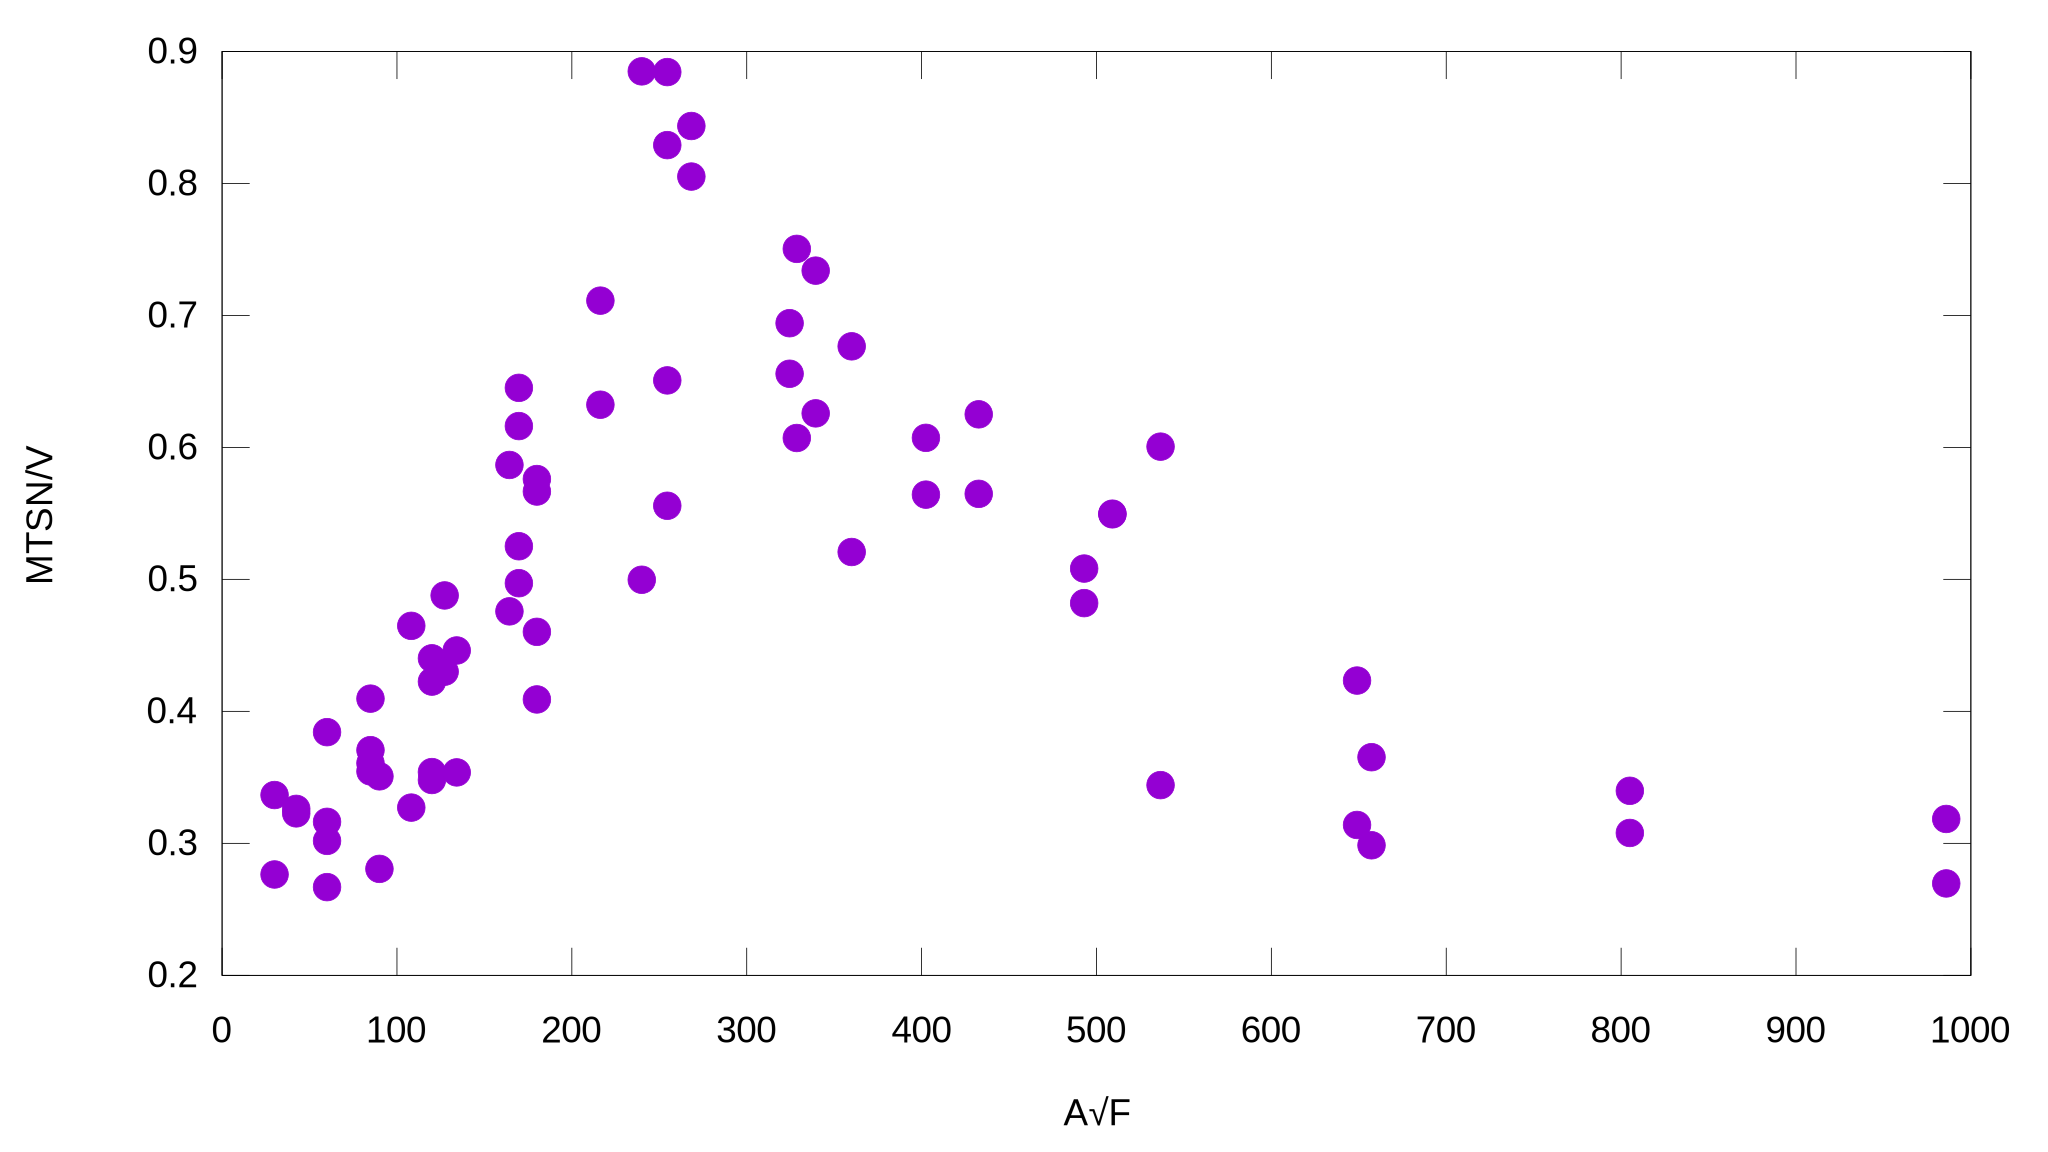
\includegraphics[width=\textwidth]{figures/ch5/asqrtFvTime}
		\caption[MTSN/V en fonction de $A\sqrt{F}$]{Moyennes des temps de sélection normalisés, divisées par la vitesse, en fonction du produit $A\sqrt{F}$, pour des cibles de vitesse moyenne ou rapide.}
		\label{fig:tAsqrtF}
	\end{figure}
	
	Celle-ci nous apprend que lorque la valeur de $A\sqrt{F}$ est autour de 250~$\degree{}Hz^{\frac{1}{2}}$, les temps de sélection sont maximaux. Nous appellerons cette valeur $PES_{max}$. De manière analogue, il est possible de considérer le produit AF, auquel cas cette valeur se trouve autour de 1200~\textdegree{}Hz. Compte tenu des résultats du chapitre 4, il est préférable d'utiliser le produit $A\sqrt{F}$.
	
	Nous pouvons donc en tirer une recommandation pratique simple : chercher à s'éloigner de ces valeurs de référence. Ainsi, la conception d'une application impliquant la sélection de cibles mobiles devrait inclure une phase d'estimation de la pseudo-entropie ou, de manière équivalente et peut-être plus pertinente, de $A\sqrt{F}$. Puis, une phase de réflexion sur les manières dont il serait possible de modifier le comportement des cibles pour s'éloigner de la valeur correspondant à la difficulté maximale.
	
	Concrètement, si la valeur de $A\sqrt{F}$ estimée est inférieure à 250, il faudra chercher à diminuer A ou F ; si elle est supérieure, il faudra chercher à les augmenter. Dans un contexte vidéoludique, par exemple, cela implique de modifier les paramètres de mouvement des objets, si cela n'a pas d'effet délétère sur les mécanismes de jeu. Dans d'autres contextes applicatifs, il n'est pas forcément aisé de modifier le comportement intrinsèque des objets.
	
	Toutefois, cette recommandation pratique vaut autant pour la conception d'applications que pour l'élaboration de techniques d'aide à la sélection. En effet, certaines des techniques de sélection étudiées dans le chapitre~\ref{chap2} sont fondées sur la modification de la taille effective des cibles ou de leur distance au curseur ; lorsqu'il s'agit de cibles mobiles, elles peuvent également agir sur la vitesse, dont nous savons que l'importance est primordiale.
	
	Dans la plupart des contextes applicatifs que nous avons étudiés, la PES d'une cible est généralement en dessous de $PES_{max}$. Pour l'en éloigner encore plus, il faut donc chercher à diminuer A et F. Bien sûr, cette diminution n'est généralement pas incompatible avec l'usage d'une autre technique d'aide à la sélection, comme par exemple le \emph{Bubble Cursor}~\cite{grossman2005bubble}, ou encore \emph{Hook}~\cite{ortega2013hook}.
	
	\subsection{Modification du paramètre V}
	Des techniques consistant à modifier la vitesse de cibles à sélectionner existent déjà, et deux d'entre elles sont présentées dans la section~\ref{sub:timeLord} : \emph{Hold}~\cite{hajri2011moving} et \emph{Target Ghost}~\cite{hasan2011comet}. La première stoppe le mouvement des cibles, tandis que la seconde ajoute à chaque cible un \emph{proxy} statique, que l'utilisateur peut sélectionner à sa place.
	
	Chacune revient en quelque sorte à arrêter le temps. La vitesse pouvant être définie comme le raport de la distance parcourue par le temps de trajet, il est logique de chercher à manipuler la vitesse en manipulant le temps. Mais jouer sur la distance est également possible, fût-ce indirectement, comme nous les verrons plus loin.
	
	\emph{Hold} a l'inconvénient d'engendrer une perte du contexte dynamique de l'application, et se prête mal aux usages en temps réel. \emph{Target Ghost} est plus souple, mais implique une forte déconnexion entre les \emph{proxies} statiques et leurs cibles-mères respectives, dont les positions deviennent totalement décorrélées.
	
	\subsubsection{\emph{Proxy} ralenti}
	Une solution moins contraignante existe, et consiste à générer un \emph{proxy} mobile, dont la vitesse est bornée par une valeur strictement inférieure à celle de la cible. À chaque instant, le \emph{proxy} se dirige vers la cible qui l'a engendré. Il apparaît immédiatement que, si le mouvement est suffisamment désordonné, même un \emph{proxy} très lent pourra suivre sa cible-mère sans que la distance entre les deux ne diverge ; pour un mouvement plus régulier, la vitesse du \emph{proxy} devra être plus proche de celle de la cible pour éviter cette divergence.
	
	Dans ce dernier cas cependant, la régularité du mouvement de la cible implique une sélection plus aisée, de sorte que le gain relativement faible apporté par l'utilisation d'un \emph{proxy} lent n'est pas nécessairement un inconvénient majeur.
	
	\begin{figure}[!htb]
		%\centering
		\begin{subfigure}[t]{0.49\textwidth}
			\centering
			\includegraphics[width=\textwidth]{figures/ch5/2_19_SpeedReduction_2_19_120_32}
			\caption{Trajectoire originale.}
			\label{fig:speedRedOriginal}
		\end{subfigure}
		~
		\begin{subfigure}[t]{0.49\textwidth}
			\centering
			\includegraphics[width=\textwidth]{figures/ch5/2_19_SpeedReduction_2_19_120_32_factor_0_75}
			\caption{Trajectoire filtrée, avec $FR = 75$~\%{}.}
			\label{fig:speedRed075}
		\end{subfigure}
		~
		\begin{subfigure}[t]{0.49\textwidth}
			\centering
			\includegraphics[width=\textwidth]{figures/ch5/2_19_SpeedReduction_2_19_120_32_factor_0_5}
			\caption{Trajectoire filtrée, avec $FR = 50$~\%{}.}
			\label{fig:speedRed050}
		\end{subfigure}
		~
		\begin{subfigure}[t]{0.49\textwidth}
			\centering
			\includegraphics[width=\textwidth]{figures/ch5/2_19_SpeedReduction_2_19_120_32_factor_0_25}
			\caption{Trajectoire filtrée, avec $FR = 25$~\%{}.}
			\label{fig:speedRed025}
		\end{subfigure}
		\caption[Utilisation de \emph{proxies} lents]{Utilisation de \emph{proxies} lents pour faciliter la sélection. Pour la trajectoire originale, V vaut 2,19~cm/s, A vaut 120\textdegree{}, F vaut 32~Hz, et chaque trajectoire est générée sur 5 secondes, comme pour les données du chapitre~\ref{chap4}. Les trois autres trajectoires sont générées avec des facteurs de ralentissement de la cible (FR) indiqués en légende de chaque sous-figure. En bleu, les trajectoires avec leurs longueurs respectives indiquées en légende ; en rouge, les aires de leurs enveloppes convexes.}
		\label{fig:speedRed}
	\end{figure}
	
	Des exemples de \emph{proxies} lents sont fournis sur la figure~\ref{fig:speedRed}. Pour les paramètres VFA étudiés ici, l'utilisation d'un \emph{proxy} limité à 75~\%{} de la vitesse de sa cible-mère permet de conserver l'allure générale de la trajectoire originale, sans trop affecter son enveloppe convexe, et en la lissant quelque peu, au point de donner une allure ciné-continue au mouvement généré (revoir la section~\ref{sub:kinematicTypes} pour la définition de ce terme). Du fait de la réduction de la vitesse et du lissage opéré, rendant le mouvement un peu plus prévisible, le \emph{proxy} est plus aisé à sélectionner.
	
	Néanmoins, l'application d'une réduction de vitesse plus forte, ne serait-ce que de 50~\%{}, introduit un décalage important entre la cible et son \emph{proxy}, ce que la forme et l'aire de l'enveloppe convexe illustrent ; le phénomène n'en est que plus marqué lorsque le facteur de réduction de vitesse est de 25~\%{}.
	
	\begin{figure}[!htb]
		\centering
		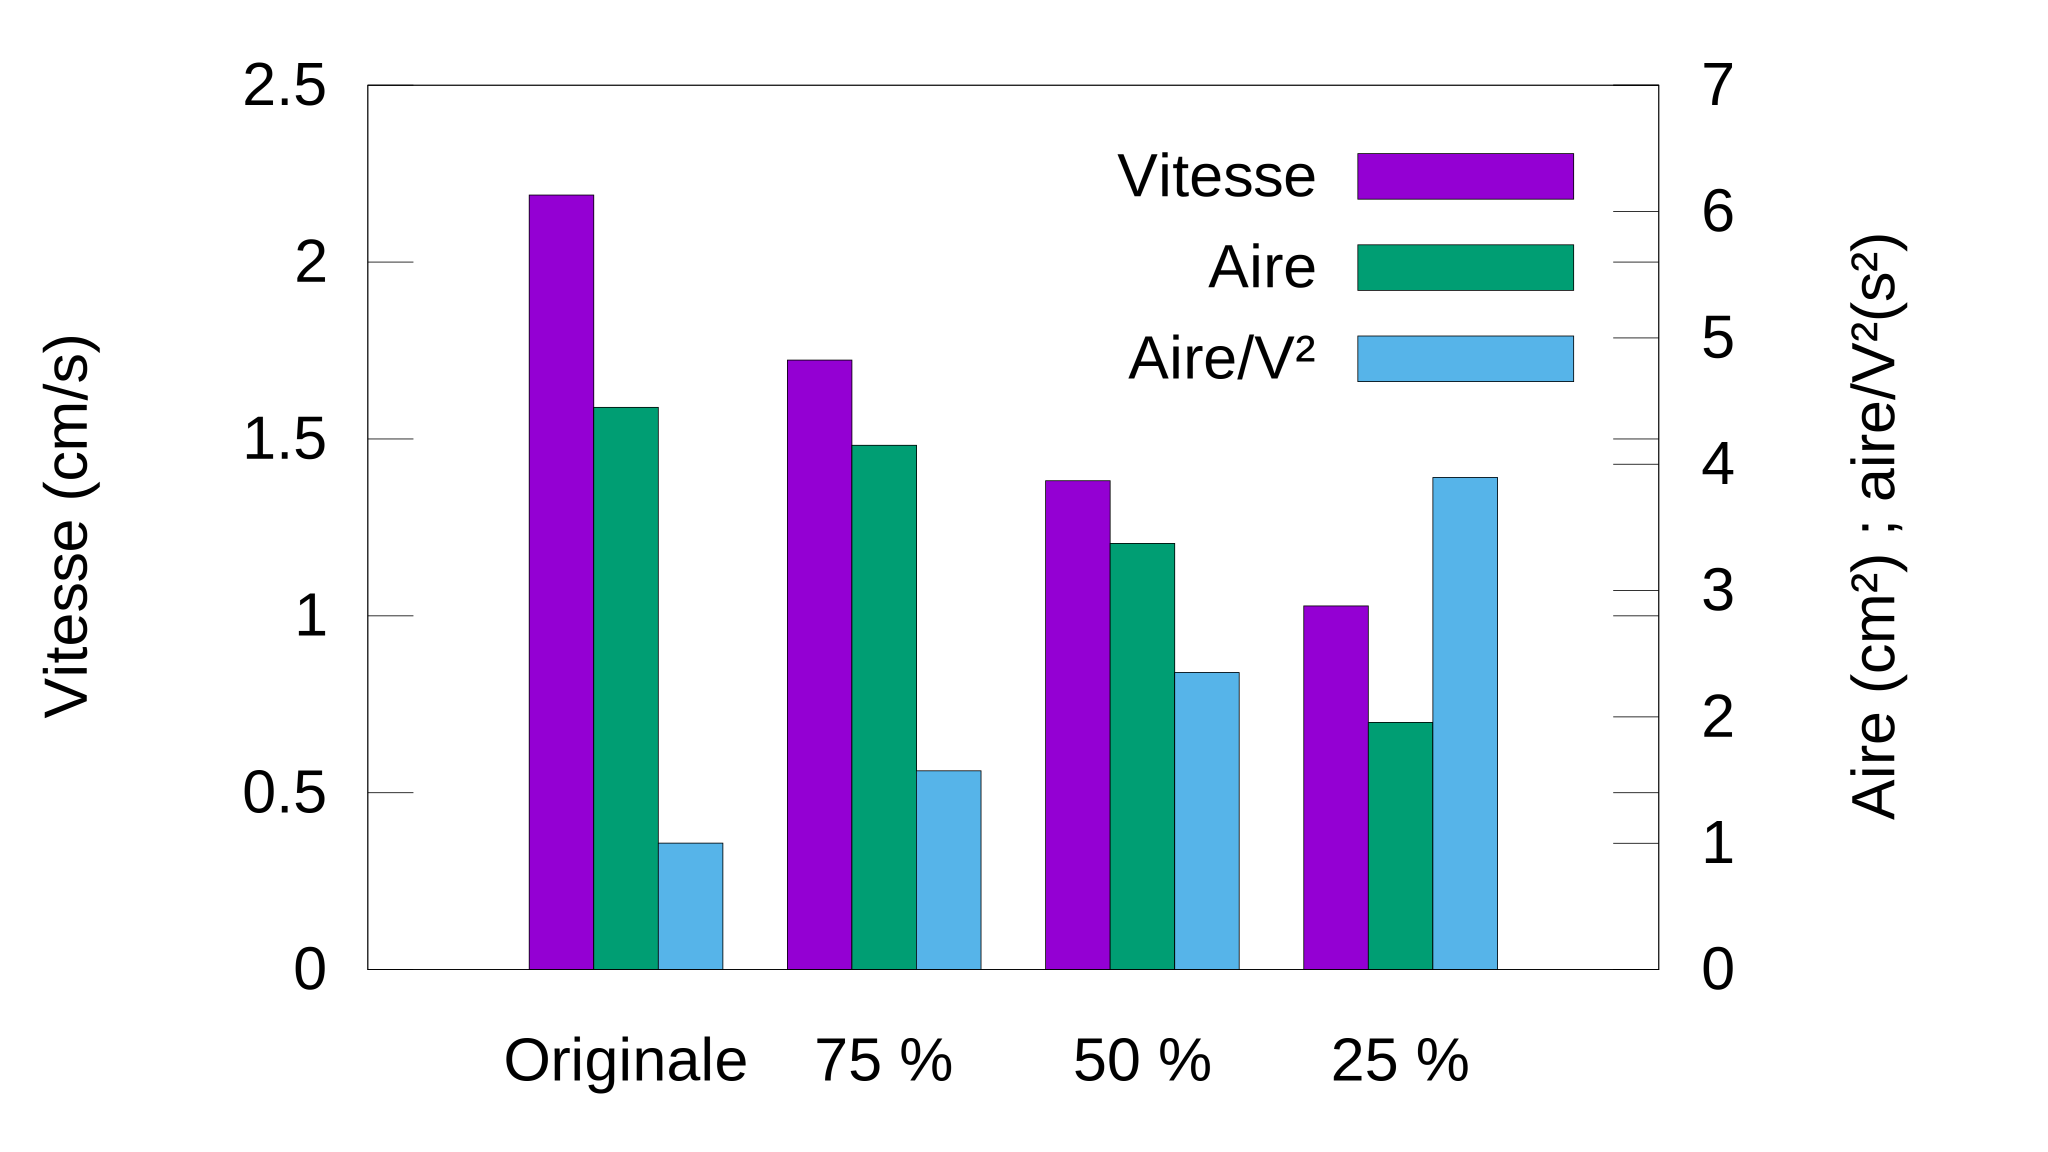
\includegraphics[width=\textwidth]{figures/ch5/filteringBySpeedRedHistograms}
		\caption[Utilisation d'un \emph{proxy} lent]{Effet de l'utilisation d'un \emph{proxy} lent sur les caractéristiques d'une trajectoire. Celle-ci est générée avec $V=2,19~cm/s$, $F=32~Hz$, et $A=120\degree{}$. La vitesse est naturellement proportionnelle au facteur de ralentissement appliqué. L'aire de l'enveloppe convexe demeure à peu près stable quand RF vaut 75~\%{}, mais chute fortement au-delà.}
		\label{fig:filteringBySpeedRed}
	\end{figure}
	
	C'est ce qu'illustre la figure~\ref{fig:filteringBySpeedRed}, sur laquelle on observe malgré tout une forte augmentation de l'aire de l'enveloppe convexe divisée par la vitesse au carré, ce qui s'explique par la diminution de la vitesse. Or, les données présentées sur la figure~\ref{fig:perf_V_RealArea_normed} (section~\ref{sub:areaVperf}) montrent que quand cette valeur est très grande, la sélection est généralement rapide. Par ailleurs, les résultats présentés sur la figure~\ref{fig:perf_V_RealArea_raw} de la même section montrent que lorsque la vitesse est faible, les temps de sélection sont toujours relativement courts de toute manière.
	
	D'autres combinaisons de VFA engendrant un mouvement plus \og brownien \fg{} toléreraient mieux de fortes réductions de vitesse, et sans doute certains contextes applicatifs seraient-ils propices à de fortes réductions, quitte à introduire un grand décalage --- potentiellement divergent --- entre une cible et son \emph{proxy}. En somme, l'utilisation d'un \emph{proxy} lent peut fortement faciliter la sélection, à condition que le contexte applicatif tolère les modifications du comportement de la cible qu'elle implique.
	
	\subsection{Modification du paramètre F}
	Il est difficile d'imaginer une façon d'augmenter la valeur de F qui ait du sens, à l'exception, peut-être, du choix d'une plus haute fréquence d'échantillonage, lorsqu'il s'agit de données mesurées ou simulées, par exemple pour un enregistrement vidéo, ou une simulation scientifique impliquant des particules.
	
	Toutefois, une option permettant de réduire le paramètre F est d'appliquer un filtrage, par exemple de façon analogue à ce qu'opérerait un filtre passe-bas. La conception d'une telle technique d'assistance à la sélection serait différente selon le degré d'intégration à l'application : avec une intégration forte, il serait possible de modifier directement le comportement des cibles ; avec une intégration faible, il faudrait se contenter d'ajouter un \emph{proxy}, comme le fait la technique \emph{Ghost}~\cite{hasan2011comet}. Ce procédé a par ailleurs l'avantage d'éviter de perdre les informations concernant les positions exactes des cibles potentielles, au prix d'un encombrement visuel accru.
	
	\subsubsection{Filtrage avec limitation à 4~Hz}
	Illustrons notre propos par un exemple concret de technique d'aide à la sélection, fondée sur une limitation de la fréquence de changements de direction à 4~Hz --- ce choix est quelque peu arbitraire, mais informé par les données de la figure~\ref{fig:fEffectPerf}, section~\ref{sub:freqEffect}. Si une cible a un paramètre F dont la valeur intrinsèque est de 32~Hz, un \emph{proxy} de la cible est créé, mais sa position n'est mise à jour que quatre fois par seconde ; les valeurs intérmédiaires étant interpolées. Cette méthode a l'avantage de permettre au \emph{proxy}, dans une certaine mesure, de \og coller \fg{} aux mouvements de la cible réelle, mais de manière moins saccadée, plus prévisible.
	
	Cela se fait toutefois au prix d'une latence inversement proportionnelle à la fréquence d'échantillonage choisie (que nous appelons $F'$), c'est-à-dire ici $\frac{1}{4}~s = 250~ms$. Naturellement, il est possible de réduire cette latence en augmentant la fréquence d'échantillonage, ce qui a l'inconvénient de diminuer l'efficacité de la technique.
	
	Cette façon de filtrer les positions des cibles permet de conserver des points en commun avec la trajectoire initiale, et donc de ne pas trop en modifier l'étendue et l'allure générale, comme l'illustre la figure~\ref{fig:filterF}.
	
	\begin{figure}[!htb]
		%\centering
		\begin{subfigure}[t]{0.49\textwidth}
			\centering
			\includegraphics[width=\textwidth]{figures/ch5/2_19_freqFilter_2_19_120_32}
			\caption{Trajectoire originale, $F = 32$~Hz.}
			\label{fig:filterFnoFilter}
		\end{subfigure}
		~
		\begin{subfigure}[t]{0.49\textwidth}
			\centering
			\includegraphics[width=\textwidth]{figures/ch5/2_19_freqFilter_2_19_120_32_filter_16}
			\caption{Trajectoire filtrée, avec $F' = 16$~Hz.}
			\label{fig:filterFw16}
		\end{subfigure}
		~
		\begin{subfigure}[t]{0.49\textwidth}
			\centering
			\includegraphics[width=\textwidth]{figures/ch5/2_19_freqFilter_2_19_120_32_filter_8}
			\caption{Trajectoire filtrée, avec $F' = 8$~Hz.}
			\label{fig:filterFw8}
		\end{subfigure}		
		~
		\begin{subfigure}[t]{0.49\textwidth}
			\centering
			\includegraphics[width=\textwidth]{figures/ch5/2_19_freqFilter_2_19_120_32_filter_4}
			\caption{Trajectoire filtrée, avec $F' = 4$~Hz.}
			\label{fig:filterFw4}
		\end{subfigure}
		\caption[Filtrage des trajectoires par limitation de fréquence]{Une trajectoire originale, et trois trajectoires produites par limitation de la fréquence. Pour la trajectoire originale, A vaut 120\textdegree{}, et chaque trajectoire est générée sur 5 secondes, comme pour les données du chapitre~\ref{chap4}. Le paramètre A n'est pas nécessairement respecté pour les trajectoires filtrées, attendu que plusieurs angles de 120\textdegree{} au plus peuvent s'accumuler d'une période à l'autre. En bleu, les trajectoires avec leurs longueurs respectives indiquées en légende ; en rouge, les aires de leurs enveloppes convexes.}
		\label{fig:filterF}
	\end{figure}
	
	\paragraph{Effet secondaire sur la vitesse des cibles.}
	Mais un effet secondaire de ce procédé est crucial : la longueur de la trajectoire est réduite. Or, attendu que la durée totale du mouvement n'est pas modifiée (elle est de 4 secondes pour les trajectoires de la figure~\ref{fig:filterF}), la vitesse moyenne de la cible diminue. Or, nous l'avons vu plus haut, la vitesse est le paramètre dont l'effet sur les temps de sélection est le plus fort, ainsi que le plus simple. En effet, les temps de sélection dépendent de la vitesse de façon approximativement affine, et les taux d'erreur, de façon approximativement linéaire (voir la figure~\ref{fig:spEffectPerf}, section~\ref{sub:spEffect}).
	
	L'effet du filtrage par fréquence sur la vitesse des cibles est illustré sur la figure~\ref{fig:filteringByFHistograms}. On y constate qu'une forte diminution de la vitesse (jusqu'à -54,34~\%{}) accompagne celle de la fréquence. L'aire de l'enveloppe convexe, elle, demeure relativement stable, avec une diminution de 14,8~\%{} seulement dans le cas le plus extrème, avec $F'=4~Hz$. Mais comme la vitesse diminue, l'aire divisée par la vitesse au carrée augmente fortement. Or, quand cette valeur est très grande, la sélection est généralement rapide, lorsque la vitesse est faible, elle l'est toujours.
	
	Il en résulte que si l'allure générale de la trajectoire, ainsi que l'espace qu'elle occupe ne changent guère, la cible devient considérablement plus aisée à sélectionner, d'après nos modèles.
		
	\begin{figure}[!htb]
		\centering
		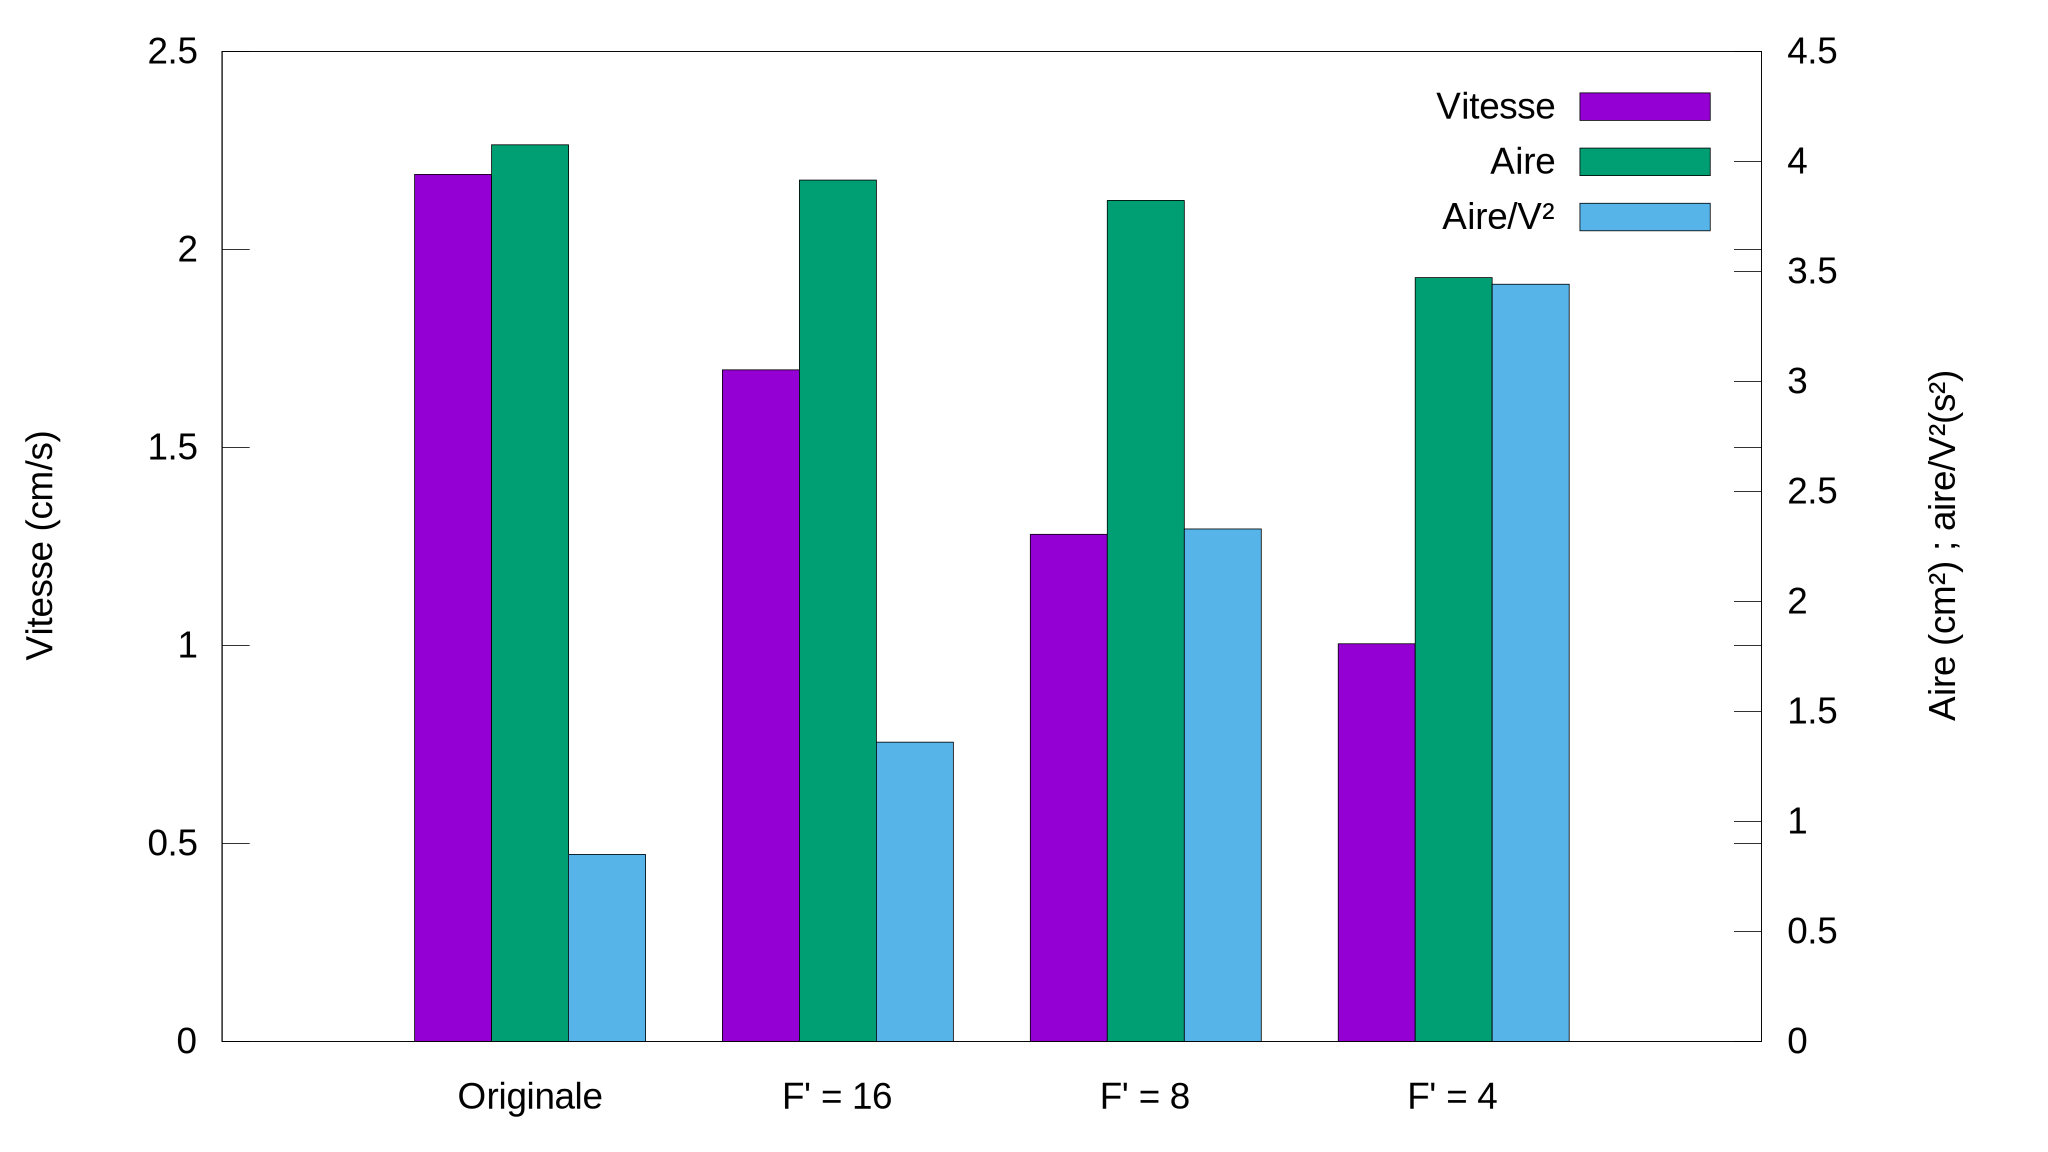
\includegraphics[width=\textwidth]{figures/ch5/filteringByFHistograms}
		\caption[Effet du filtrage fréquentiel]{Effet du filtrage fréquentiel sur les caractéristiques d'une trajectoire. Celle-ci, générée avec $V=2,19~cm/s$, $F=32~Hz$, et $A=120\degree{}$, se trouve modifiée de telle manière que la vitesse moyenne de la cible chute drastiquement --- de 2,19~cm/s à 1,00~cm/s --- de même, évidemment, que la fréquence. L'aire de l'enveloppe convexe demeure relativement stable.}
		\label{fig:filteringByFHistograms}
	\end{figure}

	Comme la figure~\ref{fig:fEffectPerf} l'illustre, la réduction de la fréquence permet d'améliorer les performances, mais que cette réduction est moins perceptible lorsque le paramètre A est particulièrement grand.

	\subsection{Modification du paramètre A}
	Dans ces cas-là, il peut être plus judicieux de chercher à diminuer ce dernier --- là encore, il paraît difficile de chercher à l'augmenter de manière sensée. La réduction du paramètre A est peut-être plus délicate que celle de F, attendu qu'elle ne se prête pas à un filtrage temporel.
	
	Certes, s'il est possible de modifier directement le comportement des objets, alors la réduction de A peut s'avérer possible dans certaines circonstances, à condition qu'elle n'ait pas d'impact trop négatif sur l'application concernée.
	
	\subsubsection{Report de la pseudo-entropie sur F}
	Pour rappel, les paramètres A et F ne sont pas égaux dans leur influence sur les performances de sélection, puisque c'est la racine carrée de F dont l'influence est primordiale, et non F lui-même. Par conséquent, il peut être judicieux de diminuer A et d'augmenter F proportionnellement, pour compenser, et maintenir une pseudo-entropie constante, si le contexte applicatif l'exige.
	
	Supposons en effet une cible dont la pseudo-entropie subjective est la \og pire \fg{} possible, soit $A\sqrt{F} = PES_{max} = 250$, avec $A = 50~; F = 25~; \sqrt{F} = 5~; AF = 1250$.
	
	S'il on veut conserver la même quantité de désordre sur une durée donnée, il faut maintenir le produit AF constant à 250. Pour ce faire, nous pouvons, par exemple, diviser A par 2, et multiplier F par le même nombre, ce qui aboutit à la situation suivante : $A = 25~; F = 50~; \sqrt{F} \approx 7,07$ ; d'où $A\sqrt{F} \approx 176,78$, soit une diminution de la PES qui l'éloigne de $PES_{max}$.
	
	Naturellement, l'effet est d'autant plus fort que le facteur choisi est élevé ; ainsi, avec 5, nous obtenons les valeurs suivantes : $A = 10~; F = 125~; \sqrt{F} \approx 11,18~; A\sqrt{F} \approx 111,80$. La figure~\ref{fig:tAsqrtF} montre que pour ces valeurs de PES, les performances de sélection sont bien meilleures que pour $PES_{max}$. Néanmoins, tous les dispositifs d'affichage ne sont pas capables d'atteindre de telles fréquences, ce qui limite la portée de cette approche.
	
	\subsubsection{Limitation de A avec compensation ultérieure}
	Une autre option consiste à imposer une limite ferme à la cible (ou à son \emph{proxy}) et à chercher à compenser à chaque nouveau changement de direction. Supposons par exemple une borne de 30\textdegree{} imposée au paramètre A, et un proxy représentant chaque cible. Pour une cible donnée, si son vecteur vitesse subit à un instant $t$ une rotation de plus de 30\textdegree{}, son \emph{proxy} ne voit son vecteur vitesse tourner que de 30\textdegree{}. Lors du prochain changement de direction du vecteur vitesse, celui du proxy est alors ajusté non pas de manière à correspondre à la nouvelle rotation subie par le vecteur vitesse réelle, mais de manière à orienter le proxy dans la direction de la cible qu'il représente, pour compenser le décalage induit par l'imposition d'une borne sur A. Cette compensation se fait néanmoins toujours avec au plus une rotation de 30\textdegree{}.
	
	Cette opération est possible sans que la distance entre la cible et son \emph{proxy} ne diverge, car les changements de direction limitent la distance totale parcourue par un objet sur une période et à une vitesse données, attendu que c'est en allant tout droit que l'on s'éloigne le plus de son point de départ.
	
	Néanmoins, selon le paramètre A intrinsèque de la cible, et selon la borne imposée, le comportement du \emph{proxy} peut-être plus ou moins déconnecté de celui de la cible potentielle qu'il représente ; aussi la prudence est-elle de mise lorsque cette technique est mise en œuvre, et il est probablement souhaitable d'éviter d'avoir un écart trop important entre la valeur originelle de A et la borne choisie. Il est toutefois possible de combiner cette imposition de borne avec le report de l'entropie sur F.
	
	\subsection{Filtrage par moyenne mobile}
	La moyenne mobile constitue un type de filtrage passe-bas assez classique. Elle consiste, pour une largeur L, à remplacer chaque valeur $x_{i}$ rencontrée dans une série par la moyenne d'un échantillon de L valeurs centré sur $x_{i}$. Là encore, une latence est introduite par le procédé, et elle est proportionnelle à L. Il serait probablement mal avisé de chercher à lisser ainsi les angles de rotation du vecteur vitesse d'une cible, car cela introduirait un décalage potentiellement divergent entre la position de la cible et celle de son \emph{proxy}.
	
	Cependant, il est possible d'appliquer un tel filtrage aux positions mêmes de la cible. Dans ce cas, la trajectoire est considérablement lissée, et ne présente plus d'angles marqués --- elle devient courbe. Ainsi, le mouvement devient ciné-continu, comme l'illustre la figure~\ref{fig:movingAverageTrajs}.
	
	\begin{figure}[!htb]
		%\centering
		\begin{subfigure}[t]{0.49\textwidth}
			\centering
			\includegraphics[width=\textwidth]{figures/ch5/2_19_MovingAverage_2_19_120_32}
			\caption{Trajectoire originale.}
			\label{fig:movAvOriginal}
		\end{subfigure}
		~
		\begin{subfigure}[t]{0.49\textwidth}
			\centering
			\includegraphics[width=\textwidth]{figures/ch5/2_19_MovingAverage_2_19_120_32_window_62_5}
			\caption{Trajectoire filtrée, avec $L = 62,5$~ms.}
			\label{fig:movAv0625}
		\end{subfigure}
		~
		\begin{subfigure}[t]{0.49\textwidth}
			\centering
			\includegraphics[width=\textwidth]{figures/ch5/2_19_MovingAverage_2_19_120_32_window_125_0}
			\caption{Trajectoire filtrée, avec $L = 125$~ms.}
			\label{fig:movAv1250}
		\end{subfigure}		
		~
		\begin{subfigure}[t]{0.49\textwidth}
			\centering
			\includegraphics[width=\textwidth]{figures/ch5/2_19_MovingAverage_2_19_120_32_window_250_0}
			\caption{Trajectoire filtrée, avec $L = 250$~ms.}
			\label{fig:movAv2500}
		\end{subfigure}
		\caption[Filtrage des trajectoires par moyenne mobile]{Une trajectoire originale, et trois trajectoires produites par application d'une moyenne mobile sur les positions de la cible. Pour la trajectoire originale, A vaut 120\textdegree{}, tandis que F est de 32~Hz. Chaque trajectoire est générée sur 5 secondes, comme pour les données du chapitre~\ref{chap4}. En bleu, les trajectoires avec leurs longueurs respectives indiquées en légende ; en rouge, les aires de leurs enveloppes convexes. Les largeurs L des fenêtres mobiles sont ici choisies avec 62,5, 125, et 250~ms, car ces durées, si ont les ramène à des fréquences, correspondent respectivement à 16, 8, et 4~Hz, soit les valeurs choisies pour illustrer le filtrage fréquentiel (figure~\ref{fig:filterF}).}
		\label{fig:movingAverageTrajs}
	\end{figure}
	
	De même que pour le filtrage fréquentiel, l'allure générale de la trajectoire, son étendue, et l'aire de son enveloppe convexe ne sont pas significativement modifiées. En revanche, si le filtrage fréquentiel tend à accentuer les angles --- et donc le caractère ciné-discret du mouvement --- la moyenne mobile produit une trajectoire \emph{lissée}, donc ciné-continue. En remplaçant les grands changement de direction instantanés par de petits changements continus, elle rend le mouvement d'une cible plus prévisible, tout en réduisant significativement sa vitesse. Le paramètres A et F n'ont donc ici plus guère de sens, à moins d'en adopter une définition plus adaptée aux mouvements ciné-continus.
	
	Ces effets sont quantifiés sur la figure~\ref{fig:filteringByMovingAverageHistograms}. Les différences sur ces métriques ne sont pas suffisamment marquées pour faire une distinction claire entre le filtrage fréquentiel et l'application d'une moyenne mobile. Cependant, les natures profondément différentes des trajectoires générées (ciné-discrètes dans le premier cas, ciné-continues dans le second) justifient la coexistence de ces deux techniques, dont chacun pourra juger de la pertinence, selon l'application visée.
	
	\begin{figure}[!htb]
		\centering
		\includegraphics[width=\textwidth]{figures/ch5/filteringByMovingAverageHistograms}
		\caption[Effet du filtrage par moyenne mobile]{Effet du filtrage par moyenne mobile sur les caractéristiques d'une trajectoire. Celle-ci, générée avec $V=2,19~cm/s$, $F=32~Hz$, et $A=120\degree{}$, se trouve modifiée de telle manière que la vitesse moyenne de la cible chute drastiquement --- de 2,19~cm/s à 1,03~cm/s lorsque la fenêtre mobile a une largeur de 250~ms. L'aire de l'enveloppe convexe demeure relativement stable.}
		\label{fig:filteringByMovingAverageHistograms}
	\end{figure}
	
	De même, un compromis entre le \og pouvoir \fg{} de lissage et la latence proportionnelle à L doit être trouvé de manière \emph{ad hoc}, selon le contexte applicatif.
	
	
	\subsection{Utilisation dynamique des proxies}
	\label{sub:dynamicProxies}
	Comme nous le précisions notamment dans la section~\ref{sub:techAug} qui évoque les techniques fondées sur l'augmentation des cibles, cette approche a l'inconvénient majeur d'accroître l'encombrement visuel, généralement d'un facteur deux lorsqu'elle implique l'utilisation de \emph{proxies}. Toutefois, il est tout à fait possible de mitiger cet impact en combinant cette approche avec de la prédiction intentionnelle. Par exemple, la technique \emph{Hook}~\cite{ortega2013hook} maintient en permanence une liste des N cibles potentielles les plus proches du curseur, où N est un entier naturel paramétrable. Ce procédé très simple pourrait être utilisé pour restreindre l'usage des \emph{proxies} : seules les N cibles en question en seraient accompagnées, les autres étant jugées trop loin du curseur pour être visées par l'utilisateur.
	
	Naturellement, selon le contexte, d'autres approches pourraient être pertinentes, comme celle d'\emph{IntenSelect}~\cite{de2005intenselect}, par exemple, fondée sur un principe similaire, mais appliqué à des rayons lancés depuis un périphérique de saisie, plutôt qu'à un curseur ponctuel. Quelle que soit l'approche exacte choisie, si le nombre de \emph{proxies} est beaucoup plus petit que le nombre total de cibles potentielles, l'encombrement visuel ajouté est faible, potentiellement inférieur à 10~\%{}, voire moins si l'on opte pour des \emph{proxies} partiellement transparents, par exemple.

	\subsection{Combinaison avec des techniques existantes}
	Les propositions détaillées ci-dessus portent sur le comportement des cibles, ou d'éventuels \emph{proxies} que l'on pourrait leur ajouter. Par conséquent, il est tout à fait possible de les combiner avec des techniques de sélection existantes, pour peu qu'elles ne consistent pas à modifier le comportement des cibles, ou du moins de le modifier de manière incompatible avec nos propositions.
	
	Les techniques fondées sur un curseur zonal ou du lancer de rayon (notamment avec désambiguïsation) peuvent être combinées avec nos propositions. Il en va de même de la sélection en cascade, ou de la prédiction de la trajectoire du curseur.
	
	Les techniques de manipulation du temps sont moins appropriées à de telles combinaisons, mais l'augmentation des objets est parfaitement possible, de même que la prédiction intentionnelle, que l'on appliquera aux seuls \emph{proxies} plutôt qu'à leurs cibles-mères.
	
	Nous recommandons donc de se rapporter à notre taxinomie des techniques de sélection (chapitre~\ref{chap2}) afin de choisir la plus approprié à chaque contexte applicatif, et de faire de même avec l'ensemble des propositions que nous détaillons dans le chapitre présent (section~\ref{sub:vfaGuide}) afin de choisir la meilleure combinaison possible. Nous suggérons par exemple de combiner le filtrage fréquentiel, qui conserve bien l'allure d'une trajectoire et son enveloppe convexe, avec la technique \emph{Hook}~\cite{ortega2013hook}, qui a fait ses preuves, mais n'est pas conçue pour gérer le mouvement brownien, que le filtrage fréquentiel permet, dans une certaine mesure, \og d'ordonner \fg{}.

\section{Estimer la difficulté de sélection pour mieux la réduire}
	Cependant, il n'est pas toujours possible de modifier le comportement des cibles. Même l'ajout de \emph{proxies} peut poser problème, y compris en en limitant le nombre par des heuristiques intentionnelles. Ces conditions ne rendent pas le modèle VFA inutile pour autant. D'une part, il permet d'estimer la difficulté de la tâche, et peut donc informer la conception de l'interface d'une application en indiquant si une aide à la sélection est nécessaire, si le nombre d'objets doit être réduit, si les objets doivent être agrandis, etc. D'autre part et surtout, il est peut-être possible d'utiliser les informations qu'il fournit pour réduire la difficulté moyenne d'une tâche de sélection.
	
	En effet, dans la plupart des contextes applicatifs évoqués au cours du chapitre~\ref{chap1}, les cibles potentielles forment un ensemble hétérogène du point de vue cinématique, c'est-à-dire que leurs mouvements respectifs ne sont pas tous de même nature. En particulier, les paramètres VFA qui les décrivent ne sont pas les mêmes.
	
	\subsection{Différents parmètres VFA, différentes difficultés}
	De fait, dans un contexte hétérogène particulier, la difficulté inhérente à la sélection d'une cible donnée n'est pas forcément la même que pour une autre cible. Or, les paramètres VFA, qui permettent d'estimer cette difficulté (notamment par le truchement de l'espérance de l'aire de l'enveloppe convexe associée, voir la figure~\ref{fig:perf_V_RealArea_better_fit} de la section~\ref{sub:areaVperf}) sont de fait différents d'une cible à l'autre, et peuvent être déterminés. Selon le contexte, ils seront déterminés exactement, ou estimés, ou mesurés en temps réel, mais ils peuvent presque toujours être connus.
	
	Il est donc possible de dresser un tableau des différentes cibles (ou des différents types de cibles) et de leurs difficultés de sélection respective, afin de savoir quels objets poseront le plus de problèmes aux utilisateurs.
	
	\subsection{Espace d'affichage et encombrement visuel}
	Bien que nous n'ayons pas spécifiquement étudié ce paramètre au cours de l'étude que nous présentons dans les section~\ref{sub:interact} et suivantes~\cite{kouyoumdjian2015characterizing}, la largeur de Fitts demeure très importante dans une tâche de sélection de cible mobile, ce qu'illustrent par ailleurs les modèles d'autres auteurs, présentés dans la section~\ref{sub:fittsMobile}. Par conséquent, augmenter la taille d'une cible mobile en facilite toujours la sélection, et des techniques conçues spécifiquement pour cette tâche sont fondées sur ce principe. C'est notamment le cas de \emph{Comet}, dont les auteurs ont confirmé l'apport empiriquement~\cite{hasan2011comet}. Il en est de même pour \emph{AttachedShock}~\cite{you2012attachedshock, you2014attachedshock}.
	
	Mais ces dernières ont l'inconvénient d'augmenter l'encombrement visuel global de la scène. Certes, il serait probablement possible d'utiliser une heuristique intentionnelle pour mitiger ce problème, comme nous le proposions pour les \emph{proxies} dans la section~\ref{sub:dynamicProxies}, en n'augmentant que les objets dont on estime qu'ils peuvent être visés par l'utilisateur. Mais l'on peut craindre que les changements de taille permanents des objets de la scène ne perturbent l'utilisateur, et nuisent au confort d'utilisation global.
	
	Plutôt que d'utiliser une heuristique intentionnelle pour choisir quelles cibles augmenter, il est possible de s'appuyer sur une estimation de la difficulté de sélection de chaque cible. Ainsi, il est possible de consacrer plus d'espace d'affichage aux objets mobiles en ayant le plus besoin.
	
	Nous proposons en effet que, dans le cadre de l'utilisation d'une technique d'augmentation des objets, il est pertinent de considérer l'espace d'affichage comme un budget, qu'il appartient au concepteur de l'application de répartir judicieusement. Il paraît logique, au moins intuitivement, d'allouer une plus grande proportion de cet espace aux cibles les plus difficiles à saisir. Plus formellement, nous émettons les hypothèses suivantes :
	
	\begin{description}
		\item[H1 :] Notre estimation de la difficulté de sélection d'une cible se montrera plus fiable que l'usage des paramètres V, F, ou A.
		\item[H2 :] Si les cibles jugées difficiles sont agrandies, et les cibles jugées faciles sont rétrécies, de sorte que l'espace d'affichage alloué à l'ensemble des cibles demeure constant, les performances de sélection mesurées sur l'ensemble des cibles sont meilleures.
	\end{description}
	
	Ici, une cible \og jugée difficile \fg{} est une cible pour laquelle notre modèle prédit un temps de sélection relativement élevé, tandis qu'une cible \og jugée facile \fg{} a un temps de sélection prédit relativement faible (voir la figure~\ref{fig:perf_V_RealArea_better_fit} de la section~\ref{sub:areaVperf}).
	
	\subsection{Expérience et protocole}
	Afin d'évaluer notre hypothèse H1, nous avons mené une étude empirique avec 16 sujets, au cours de laquelle il leur était demandé de sélectionner des cibles rondes en cliquant dessus, dans un environnement homogène d'une part, et hétérogène de l'autre --- c'est-à-dire avec des cibles mues par les mêmes paramètres VFA et, respectivement, par des paramètres différents.
	
	Dans la condition hétérogène, chaque cible est de même taille ; dans la condition hétérogène, elles sont de tailles différentes selon l'estimation de leur difficulté de sélection, faite à partir de leurs paramètres VFA.
	
	\subsection{Dispositif expérimental et sujets}
	Chaque sujet ayant participé à l'étude l'a fait avec une machine identique : un ordinateur de bureau doté d'un écran de 24 pouces de diagonale, et d'une souris optique filaire ambidextre, sans accélération du curseur.
	
	Les sujets étaient assis sur des chaises de bureau, et avaient la possibilité d'ajuster la luminosité et le contraste de l'écran, selon leurs préférences personnelles, afin de garantir leur confort.
	
	Notre groupe de 17 sujets était constitué de 16 hommes et 1 femme, de 16 droitiers et 1 gaucher, son âge moyen est de 22 ans, avec un écart-type d'un peu plus de 4 ans.
	
	\subsection{Tâche et conditions}
	L'application utilisée pour mener l'étude affiche des disques en bleu sur un fond noir rectangulaire, de dimensions 49,6~cm$\times$27,9~cm, cerné d'un cadre gris. À tout moment, l'objet à sélectionner est rouge, tandis que les distracteurs demeurent bleus. Une fois que la cible est sélectionnée avec succès (c'est-à-dire une fois que le sujet a cliqué dessus), elle redevient bleue, et une autre devient rouge. Dans la condition homogène, chaque cible mesure 19,2~mm de diamètre.
	
	De surcroît, chaque nouvelle cible est repositionnée dès qu'elle devient rouge, à une distance par rapport au curseur précisément réglée sur 13,95~cm, dans une direction par rapport au curseur choisie de manière aléatoire, à une exception près : si la direction choisie implique une sortie du cadre noir servant de fond, une autre direction est choisie aléatoirement --- cette opération pouvant éventuellement être répétée plusieurs fois, jusqu'à ce qu'une position convenable soit trouvée. Ce déplacement soudain n'a été remarqué par aucun des sujets, sans doute parce qu'il a lieu à un moment où le sujet se concentre sur autre chose (la cible précédente qu'il vient de réussir à sélectionner) et parce que le changement de couleur, du bleu vers le rouge vif, fait distraction.
	
	La figure~\ref{fig:evalAppRunning} fournit des illustrations de l'application en cours d'exécution, dans sa condition homogène (figure~\ref{fig:homoRunning}), et dans sa condition hétérogène (figure~\ref{fig:heteroRunning}). Contrairement à la précédente étude, nous avons cherché à nous approcher des conditions d'une application \og réelle \fg{}, c'est-à-dire en plein écran. De fait, les dimensions et vitesses sont plus élevées, d'autant que nous avons souhaité nous concentrer sur les conditions les plus difficiles.
	
	\begin{figure}[!htb]
		%\centering
		\begin{subfigure}[t]{\textwidth}
			\centering
			\includegraphics[width=\textwidth]{figures/ch5/homoRunning}
			\caption{Condition homogène : toutes les cibles font la même taille.}
			\label{fig:homoRunning}
		\end{subfigure}
		~
		\begin{subfigure}[t]{\textwidth}
			\centering
			\includegraphics[width=\textwidth]{figures/ch5/heteroRunning}
			\caption{Condition hétérogène : les cibles sont de tailles différentes.}
			\label{fig:heteroRunning}
		\end{subfigure}
		\caption[Application pour l'évaluation, homogène vs. hétérogène]{Application utilisée pour mener notre étude, dans ses conditions homogène et hétérogène. Les distracteurs sont en bleu, la cible est en rouge, et la barre verte au bas de l'écran indique le taux de complétion de l'évaluation.}
		\label{fig:evalAppRunning}
	\end{figure}
	
	\subsubsection{Conditions}
	Pour la condition d'entrainement, toutes les combinaisons des paramètres VFA suivants étaient évaluées, 5 fois chacune :
	
	\begin{description}
		\item[V :] 9,3 ; 15,5~cm/s (2 valeurs)
		\item[F :] 4 ; 16 ; 32~Hz (3 valeurs)
		\item[A :] 45 ; 90 ; 180\textdegree{} (3 valeurs)
	\end{description}
	
	À ces combinaisons s'ajoutaient une condition de mouvement totalement rectiligne à 15,5~cm/s, répétée 10 fois. Au total, il y avait donc $2\times{}3\times{}3\times{}5+1\times{}10=100$ essais. La session d'entraînement était menée dans la condition homogène seulement, afin d'en limiter la durée. Ce choix peut biaiser quelque peu les résultats en faveur de la condition homogène, bénéficiant potentiellement d'un effet d'entraînement plus marqué.
	
	Pour les conditions homogène et hétérogène, nous avions toutes les combinaisons suivantes, évaluées 6 fois au lieu de 5 :
	
	\begin{description}
		\item[V :] 3 ; 5 (2 valeurs)
		\item[F :] 4 ; 8 ; 16 ; 32~Hz (4 valeurs)
		\item[A :] 45 ; 90 ; 180\textdegree{} (3 valeurs)
	\end{description}
	
	Là aussi, une condition de mouvement rectiligne à 15,5~cm/s était ajoutée, et répétée 12 fois. Au total, il y avait donc $2\times{}4\times{}3\times{}6+1\times{}12=156$ essais.
	
	Nous avons choisi ces valeurs en nous appuyant sur les enseignements de l'étude décrite dans le chapitre~\ref{chap4}. En effet, il importe d'avoir suffisamment d'essais par condition pour obtenir des résultats précis, tout en limitant la durée de chaque passation, afin d'éviter de trop fatiguer ou lasser nos sujets. Il importe également d'échantillonner correctement notre espace des paramètres afin de ne pas omettre de \og type \fg{} ou \og famille \fg{} de mouvement importants\ldots{}
	
	Il convient donc d'éliminer les paramètres qui ne sont pas indispensables, et d'essayer d'augmenter le nombre d'essais par condition. En particulier, nous avions constaté que les cibles lentes étaient toujours relativement aisées à sélectionner ; nous les avons donc supprimées. L'analyse de nos précédentes données montre également une certaine continuité dans l'effet du paramètre F, et suggère fortement que sa racine carrée soit à prendre en compte, plus que F lui-même. De plus, nous avons observé que les très basses fréquences génèrent du mouvement relativement prévisible et aisé à sélectioner.
	
	Par conséquent, nous avons opté pour un échantillonnage exponentiel, avec 4 valeurs différentes, au lieu des 7 de la précédente étude, en omettant les plus faibles.
	
	De même, nos résultats montraient que le mouvement rectiligne était toujours aisé à sélectionner, aussi avons-nous supprimé la valeur 0 de l'ensemble des valeurs de A, en conservant tout de même 12 essais rectilignes. Pour réduire le nombre de conditions, nous avons remplacé les valeurs 30 et 60 par 45, et supprimé la valeur 120. Ceci nous a permis de passer de 6 valeurs de A à seulement 4.
	
	\emph{In fine}, cette révision des valeurs des paramètres VFA nous a permis de passer de $3\times{}7\times{}6+1=126$ combinaisons différentes à seulement $2\times{}4\times{}3+1=26$. En revanche, nous avons augmenté le nombre d'essais par combinaison, passant de 4 à 6, ou 12 pour la condition rectiligne (répétée 20 fois dans l'étude précédente). Ainsi, nous obtenons $24\times{}6+12=156$ essais au lieu de $126\times{}4+20=524$ précédemment. Toutefois, chaque sujet était soumis à deux conditions différentes, pour un total de 312 essais. 
	
	Cette réduction du nombre total d'essais nous parut appropriée, compte tenu d'une part des remarques des sujets de notre première étude, et d'autre part de l'augmentation de la difficulté moyenne des sélections dans cette seconde expérience, du fait de la suppression des vitesses faibles, et de l'augmentation des valeurs retenues, même si l'agrandissement des cibles compense partiellement.
	
	\subsection{Procédure et collecte des données}
	L'expérience à proprement parler était précédée d'une session d'entraînement, décrite ci-dessus.
	
	Ensuite, et avant de débuter les sélections, un très bref questionnaire était soumis à chaque sujet. Les questions suivantes y étaient posées (voir la figure~\ref{fig:questionnaire}) :
	
	\begin{itemize}
		\item Quel est votre nom ?
		\item Êtes-vous une homme ou une femme ?
		\item Êtes-vous droitier ou gaucher ?
		\item Quel âge avez-vous ?
		\item À quelle fréquence jouez-vous aux jeux vidéo ? (Jamais -- rarement -- parfois -- souvent -- tous les jours).
	\end{itemize}
	
	\begin{figure}[!htb]
		\centering
		\includegraphics[width=\textwidth]{figures/ch5/questionnaire}
		\caption[Questionnaire]{Questionnaire soumis aux sujets de notre étude empirique, avant l'étude elle-même.}
		\label{fig:questionnaire}
	\end{figure}
	
	Les sujets devaient ensuite actionner la barre d'espace pour lancer l'expérience. La moitié (9) d'entre eux a complété la condition homogène d'abord, et hétérogène ensuite ; l'autre moitié (8) a complété ces conditions dans l'ordre inverse, afin de compenser d'éventuels effets d'apprentissage, par ailleurs palliés par la session d'entrainement préliminaire.
	
	Afin de tenter d'harmoniser les stratégies de sélection de nos sujets (c'est-à-dire de les rapprocher les unes des autres sur le continuum précision-vitesse), nous leur avons fourni pour consigne de tâcher de sélectionner chaque cible en moins de 10 essais. Cette valeur, délibérément élevée, fut choisie pour inciter les sujets à privilégier la vitesse, afin de réduire le temps de sélection par essai, et donc d'améliorer le ratio $\frac{nombre~d'essais}{durée~de~l'expérience}$, attendu que la durée de l'expérience tend à augmenter la fatigue et la lassitude des sujets, surtout pour une tâche aussi répétitive et nécessitant un tel degré de concentration.
	
	Afin de limiter cette fatigue et cette lassitude, nous imposons une pause après la sélection de 25~\%{} des cibles, ainsi qu'après 50~\%{} et 75~\%{} d'entre elles. Chaque sujet est libre de laisser la pause durer aussi longtemps qu'il le souhaite, afin de récupérer pleinement. Une pression de la barre d'espace permet de reprendre les sélections de cibles.
	
	Une barre de progression affichant le taux de complétion de l'expérience est affichée en permanence au bas de l'écran, en vert, et lorsque tous les essais ont été effectués, un message s'affiche pour indiquer la fin de l'expérience et remercier les sujets.
	
	\subsection{Ajustement des tailles des cibles}
	Pour déterminer la taille optimale de chaque cible, nous nous sommes appuyés sur le modèle que nous proposions dans la section~\ref{sub:areaVperf}, en le simplifiant pour le rendre plus commode à utiliser. Nous utilisons toujours la même équation pour calculer l'espérance de l'aire de l'enveloppe convexe d'une cible, que nous reproduisons dans le chapitre présent, équation~\ref{eq:ch5areaModel}.
	
	\begin{equation}
		\mathbb{E}(\mathcal{A}(ec)) = V^{2}N \left( A\sqrt{F} \right)^n \left(1+\left(\frac{A\sqrt{F}}{x_n}\right)^{|\beta|s}\right)^{\frac{\operatorname{sgn}(\beta)}{s}}
		\label{eq:ch5areaModel}
	\end{equation}
	
	Nos précédents travaux nous permettent de supposer qu'une parabole \og inversée \fg{} (i.e. croissante, puis décroissante) fonction de $\mathbb{E}(\mathcal{A}(ec))$ fournit une approximation utile du temps de sélection d'une cible (voir la figure~\ref{fig:perf_V_RealArea_better_fit}, section~\ref{sub:areaVperf}). Il est donc possible, sur le principe, d'utiliser la valeur de cette parabole comme facteur d'agrandissement/rétrécissement d'une cible. En l'état, toutefois, cette parabole présente quelques inconvénients.
	
	Premièrement, ses valeurs, entièrement comprises dans l'intervalle [0,05 ; 0,35] ne fournissent pas des facteurs directement utilisables. Deuxièmement, l'application de tels facteurs mènerait à un rétrécissement de toutes les cibles qui, même s'il était compensé par un agrandissement uniforme après (i.e. appliquant le même facteur à toutes les cibles) ne garantirait pas la constance de la somme des aires de toutes les cibles. Troisièmement, l'intervalle d'antécédents pour lesquels la parabole est utile, et son point de symmétrie ne sont pas clairs. Enfin, il n'est pas évident que le facteur d'agrandissement d'une cible doive être proportionnel à l'estimation du temps de sélection --- peut-être une parabole plus \og plate \fg{} fournirait-elle de meilleurs résultats, ou, au contraire, peut-être une parabole plus \og aiguë \fg{} serait-elle plus appropriée.
	
	Nous avançons donc qu'une bonne fonction d'ajustement des tailles devrait :
	
	\begin{itemize}
		\item Être parabolique, croissante, puis décroissante,
		\item Être utile sur l'intervalle [0 ; 1], avec un maximum en 0,5 qui soit également son point de symmétrie,
		\item Être ajusteable à l'aide d'un paramètre simple, afin d'être plus ou moins plate ou aiguë,
		\item Ne pas modifier la somme des aires de toutes les cibles --- ce qui est équivalent au fait que l'intégrale de la fonction vaille 1 sur l'intervalle [0 ; 1].
	\end{itemize}
	
	\subsubsection{Parabole inversée d'intégrale unitaire}
	Nous proposons donc la fonction de l'équation~\ref{eq:scalingParabola}, qui remplit tous les critères :
	
	\begin{equation}
		p(N,x) = \frac{1}{1-\frac{N}{12}} \left(1-N\left(x-\frac{1}{2}\right)^2\right)
		\label{eq:scalingParabola}
	\end{equation}
	
	La figure~\ref{fig:parabolae} illustre le comportement de cette fonction sur l'intervalle [0 ; 1] en fonction de la valeur de N, librement choisie entre 0 et 4. Celle-ci permet d'ajuster l'allure de la parabole, et donc la mesure dans laquelle ce procédé agrandit les cibles \og difficiles \fg{} et rétrécit les cibles \og faciles \fg{}. Pour un effet prononcé, on optera donc pour une valeur proche de 4, tandis que l'on préférera une valeur proche de 0 pour un effet plus léger.
	
	Attention toutefois, la constance de la somme des aires de toutes les cibles n'est garantie que si celles-ci sont réparties uniformément sur l'intervalle normalisé de leurs aires\footnotemark{}. En pratique, ce n'est généralement pas le cas, et une légère correction doit s'appliquer. Pour cela, nous mesurons cette somme des aires avant l'ajustement des tailles, puis après, et appliquons un petit correctif uniforme à la hausse ou à la baisse, selon le cas rencontré. Ce correctif permet aussi d'appliquer le facteur d'ajustement de taille non pas à l'aire d'une cible mais, dans un souci de simplicité, au rayon de chaque cible.
	
	\footnotetext{La normalisation doit se faire par rapport au maximum d'espérance de l'aire d'une enveloppe convexe de trajectoire, correspondant à $A\sqrt{F} = 120$.}
	
	\begin{figure}[!htb]
		%\centering
		\begin{subfigure}[t]{0.49\textwidth}
			\centering
			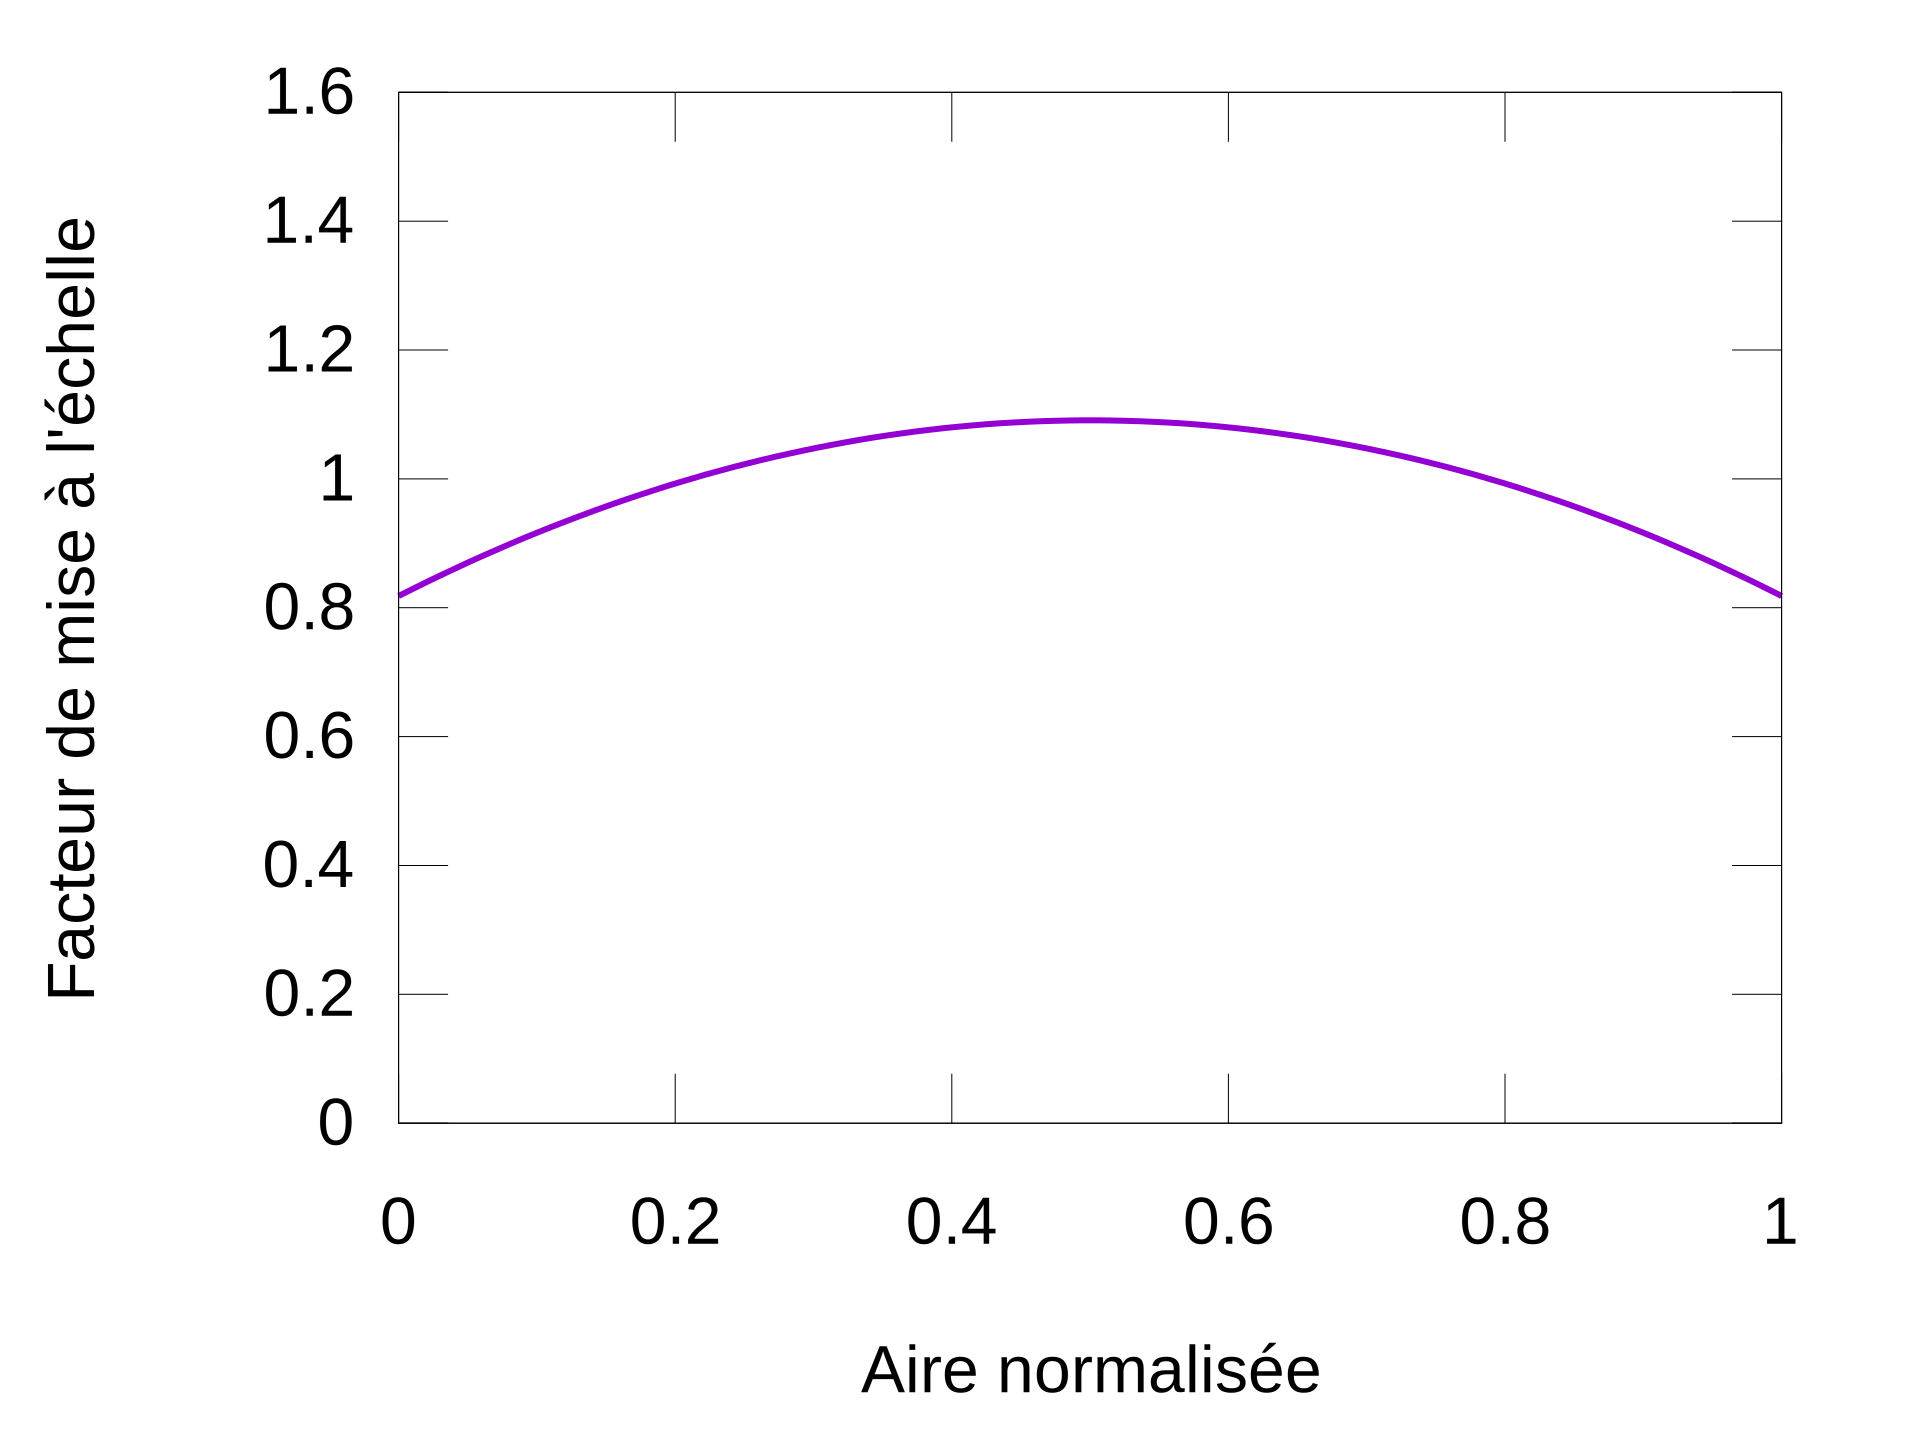
\includegraphics[width=\textwidth]{figures/ch5/parabola1}
			\caption{$N=1$.}
			\label{fig:parabola1}
		\end{subfigure}
		~
		\begin{subfigure}[t]{0.49\textwidth}
			\centering
			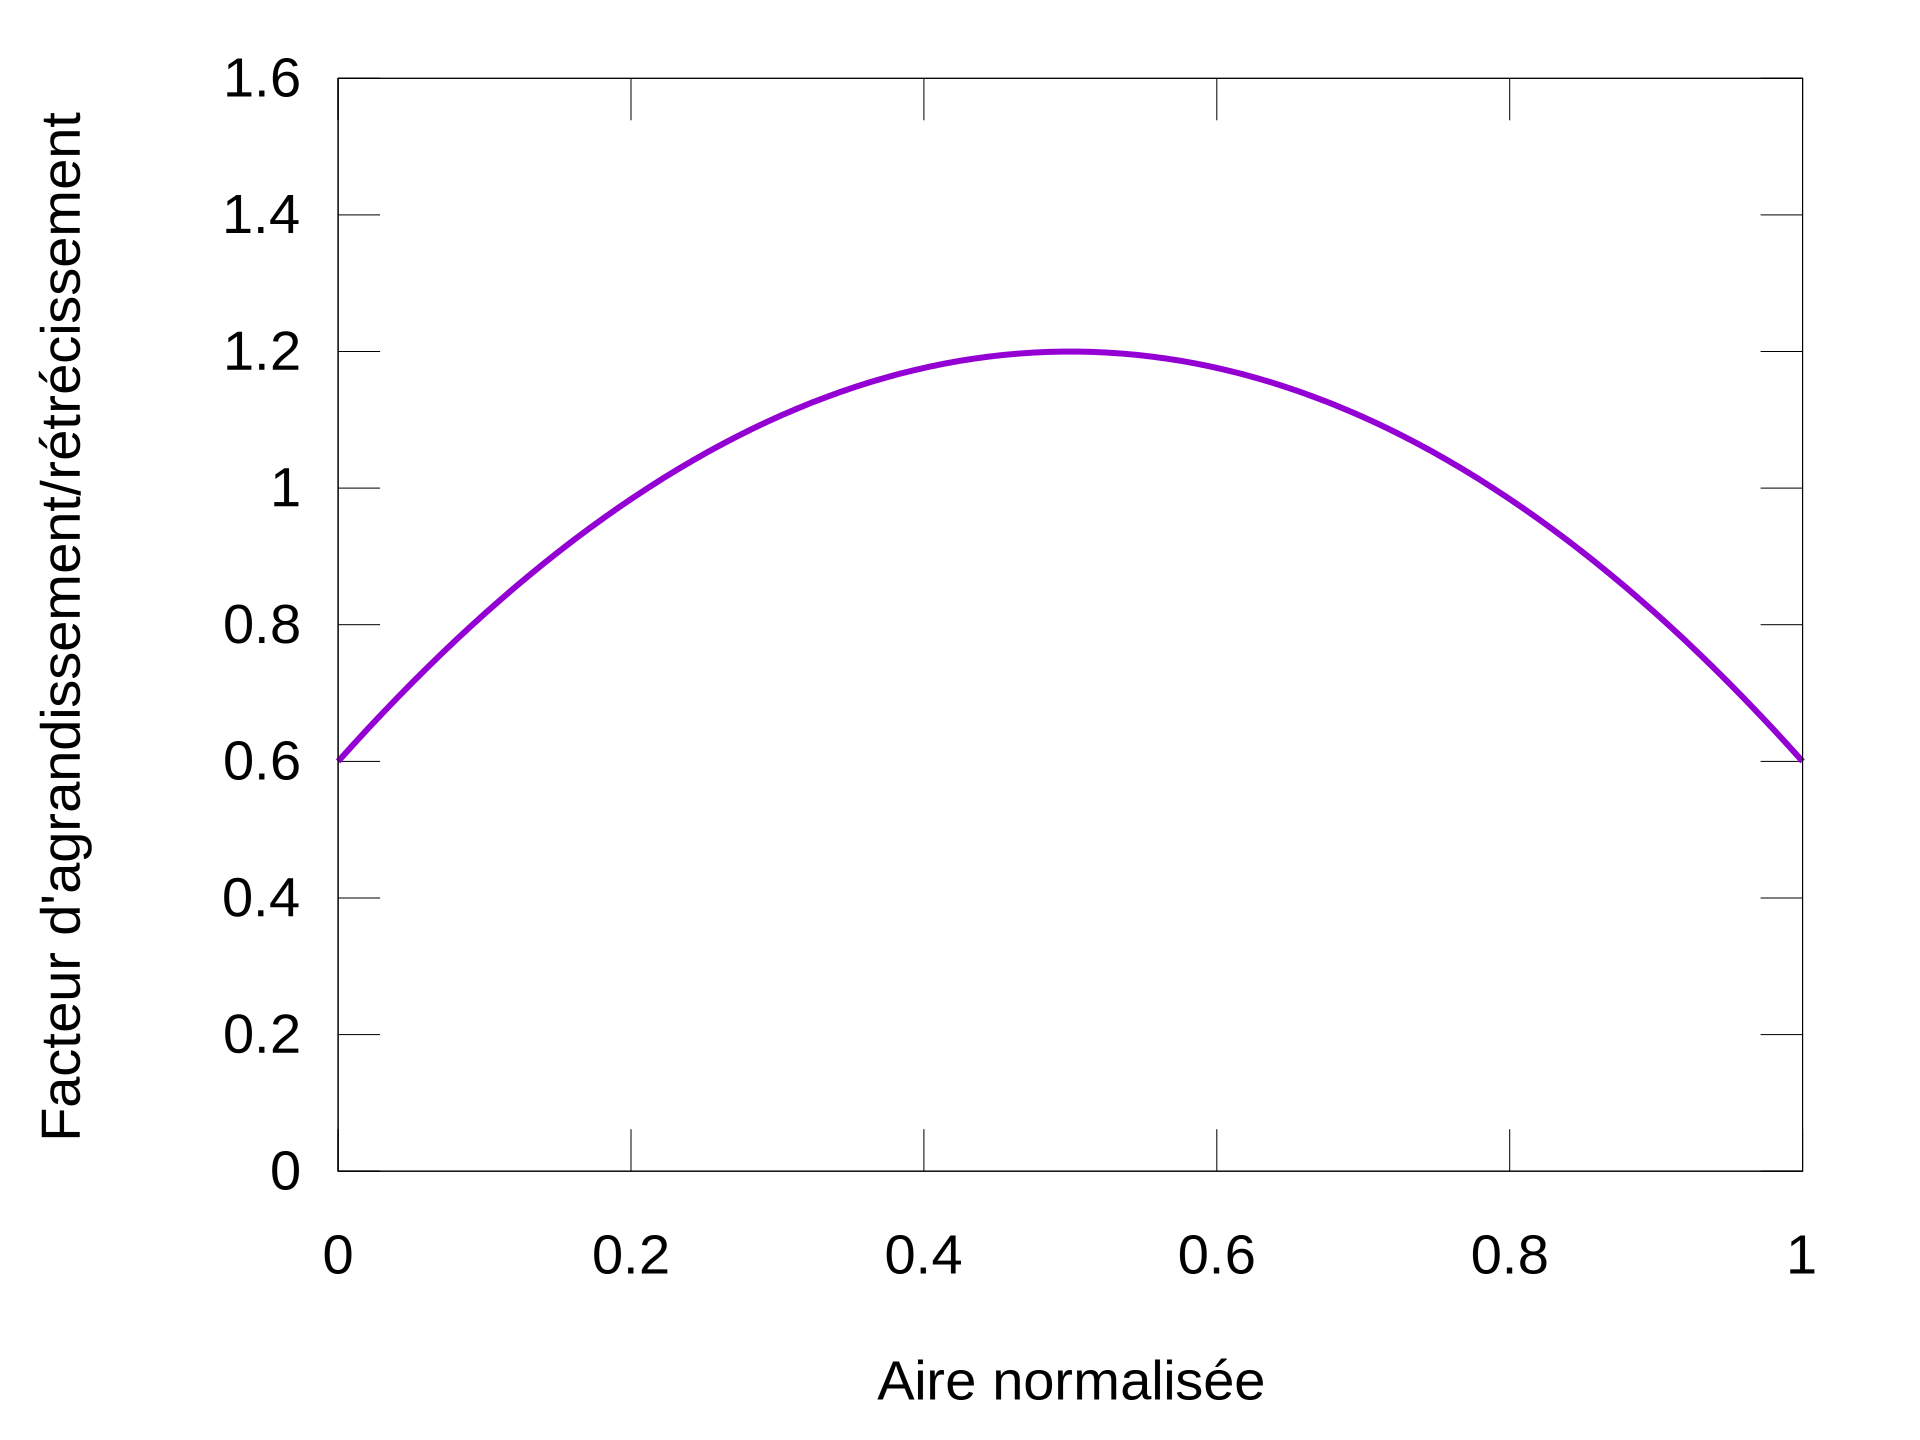
\includegraphics[width=\textwidth]{figures/ch5/parabola2}
			\caption{$N=2$.}
			\label{fig:parabola2}
		\end{subfigure}
		~
		\begin{subfigure}[t]{0.49\textwidth}
			\centering
			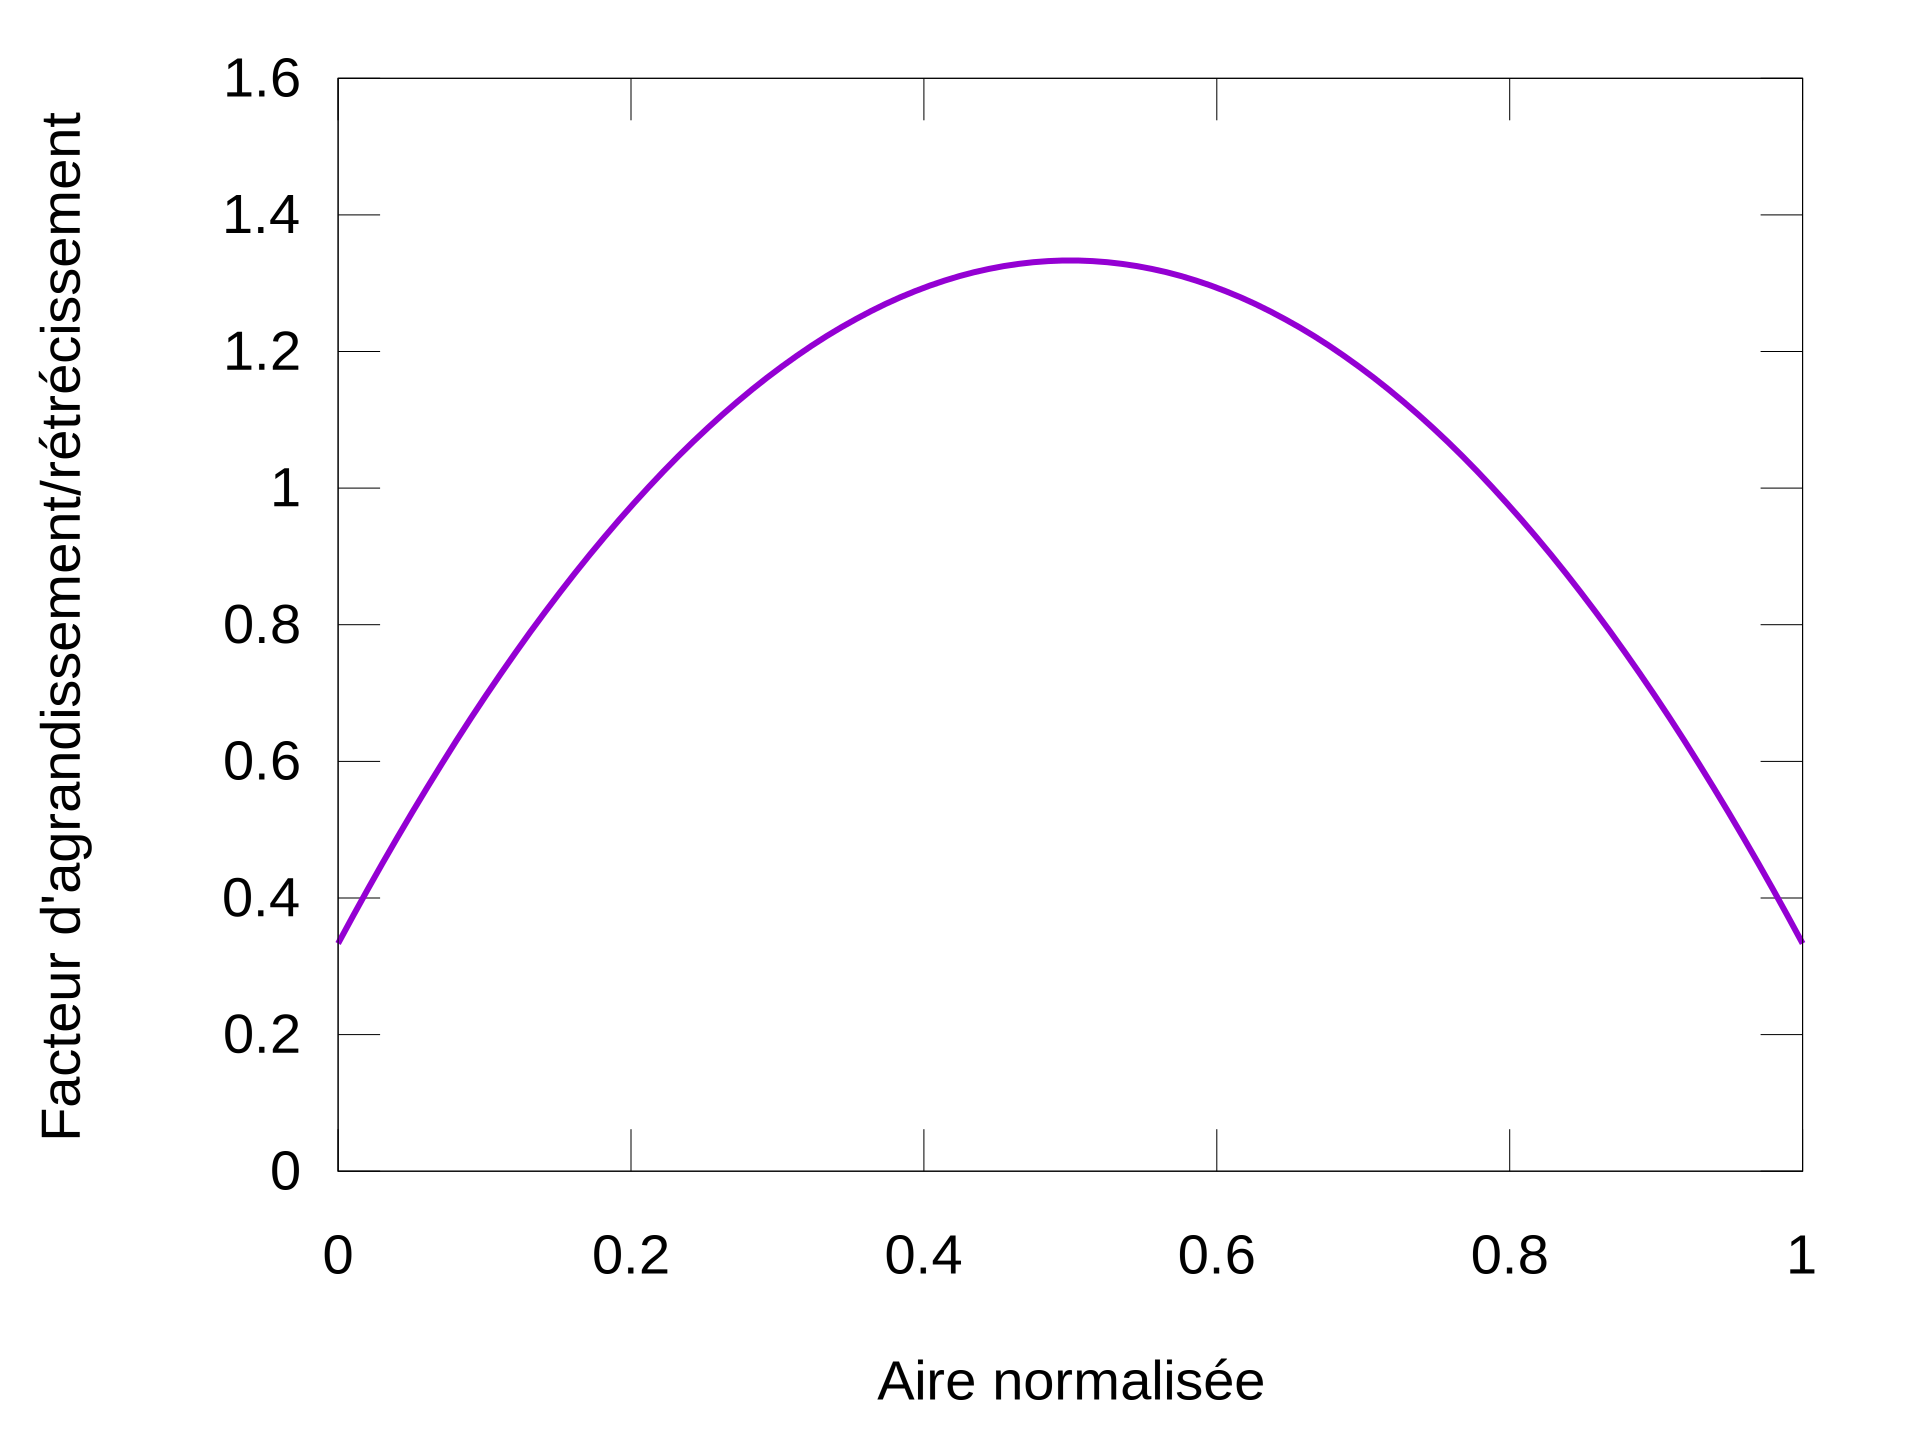
\includegraphics[width=\textwidth]{figures/ch5/parabola3}
			\caption{$N=3$.}
			\label{fig:parabola3}
		\end{subfigure}		
		~
		\begin{subfigure}[t]{0.49\textwidth}
			\centering
			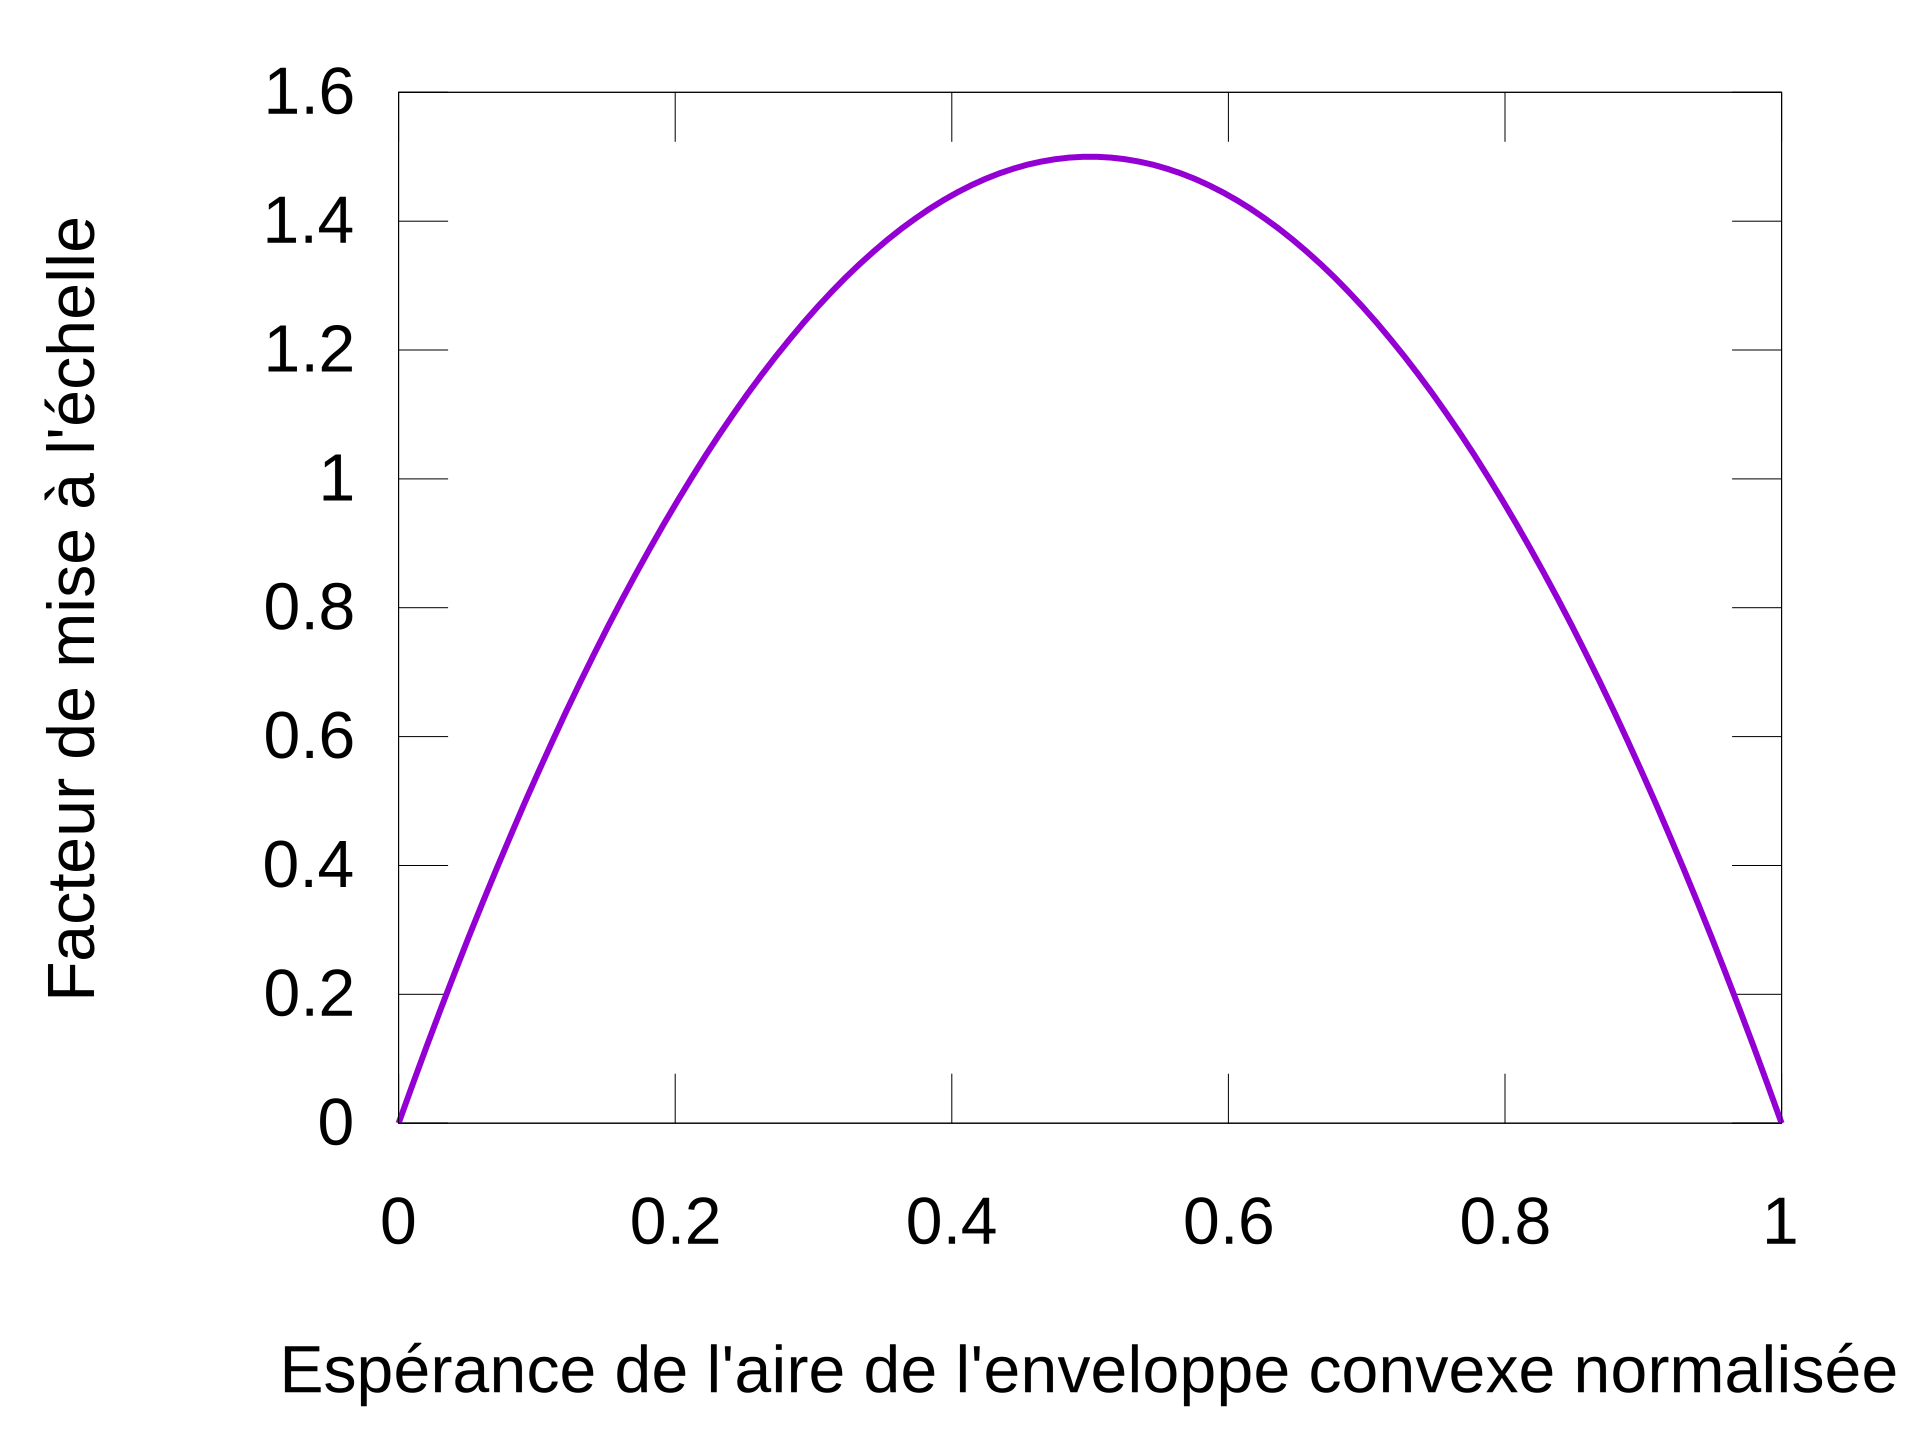
\includegraphics[width=\textwidth]{figures/ch5/parabola4}
			\caption{$N=4$.}
			\label{fig:parabola4}
		\end{subfigure}
		\caption[Paraboles pour ajuster les tailles des cibles]{Paraboles pour ajuster les tailles des cibles.}
		\label{fig:parabolae}
	\end{figure}
	
	À l'issue de plusieurs pilotes, nous avons choisi la valeur $N=2$. Ce choix informé par des essais empiriques n'est pas nécessairement optimal.
	
	\subsubsection{Données collectées}
	Nous avons collecté de nombreuses données, certaines sont constantes, d'autres sont liées à des événements ou synthétiques, et certaines changent à chaque tour de boucle du logiciel d'évaluation, c'est-à-dire 60 fois par seconde.
	
	Les données constantes sont les suivantes :
	
	\begin{itemize}
		\item Les paramètres VFA de chaque cible ;
		\item L'espérance de l'aire de l'enveloppe convexe de chaque cible, d'après ses paramètres VFA ;
		\item L'estimation de la difficulté de sélection de chaque cible, d'après notre modèle.
	\end{itemize}
	
	Les données liées à des événements ou synthétiques sont les suivantes :
	
	\begin{itemize}
		\item Le temps de sélection de chaque cible, pour chaque essai ;
		\item Le nombre d'erreur pour chaque cible, pour chaque essai.
	\end{itemize}
	
	Les données collectées à chaque tour de boucle sont les suivantes :
	
	\begin{itemize}
		\item Le temps écoulé depuis le début de l'expérience (pauses exclues) ;
		\item La position de chaque cible dans les coordonnées du monde ;
		\item La position de chaque cible dans les coordonnées de l'écran ;
		\item La direction de chaque cible dans les coordonnées de l'écran ;
		\item La position du curseur dans les coordonnées du monde ;
		\item La position du curseur dans les coordonnées de l'écran ;
		\item La cible que l'utilisateur est actuellement censé sélectionner (celle qui est rouge) ;
		\item Une valeur booléenne indiquant si l'utilisateur a cliqué sur sa souris pendant la dernière \emph{frame} ;
		\item Une valeur booléenne indiquant si l'utilisateur a cliqué sur la cible rouge pendant la dernière \emph{frame} ;
		\item Le nombre d'erreurs pendant la dernière \emph{frame}.
	\end{itemize}
	
	\subsection{Résultats}
	Les données collectées les plus importantes sont les temps de sélection, et les erreurs. Nous allons dans un premier temps les examiner séparément, puis ensemble.
	
	\begin{figure}[!htb]
		%\centering
		\begin{subfigure}[t]{0.49\textwidth}
			\centering
			\includegraphics[width=\textwidth]{figures/ch5/timeRes}
			\caption{Temps moyens de sélection, et intervalles de confiance à 95~\%{}.}
			\label{fig:timeRes}
		\end{subfigure}
		~
		\begin{subfigure}[t]{0.49\textwidth}
			\centering
			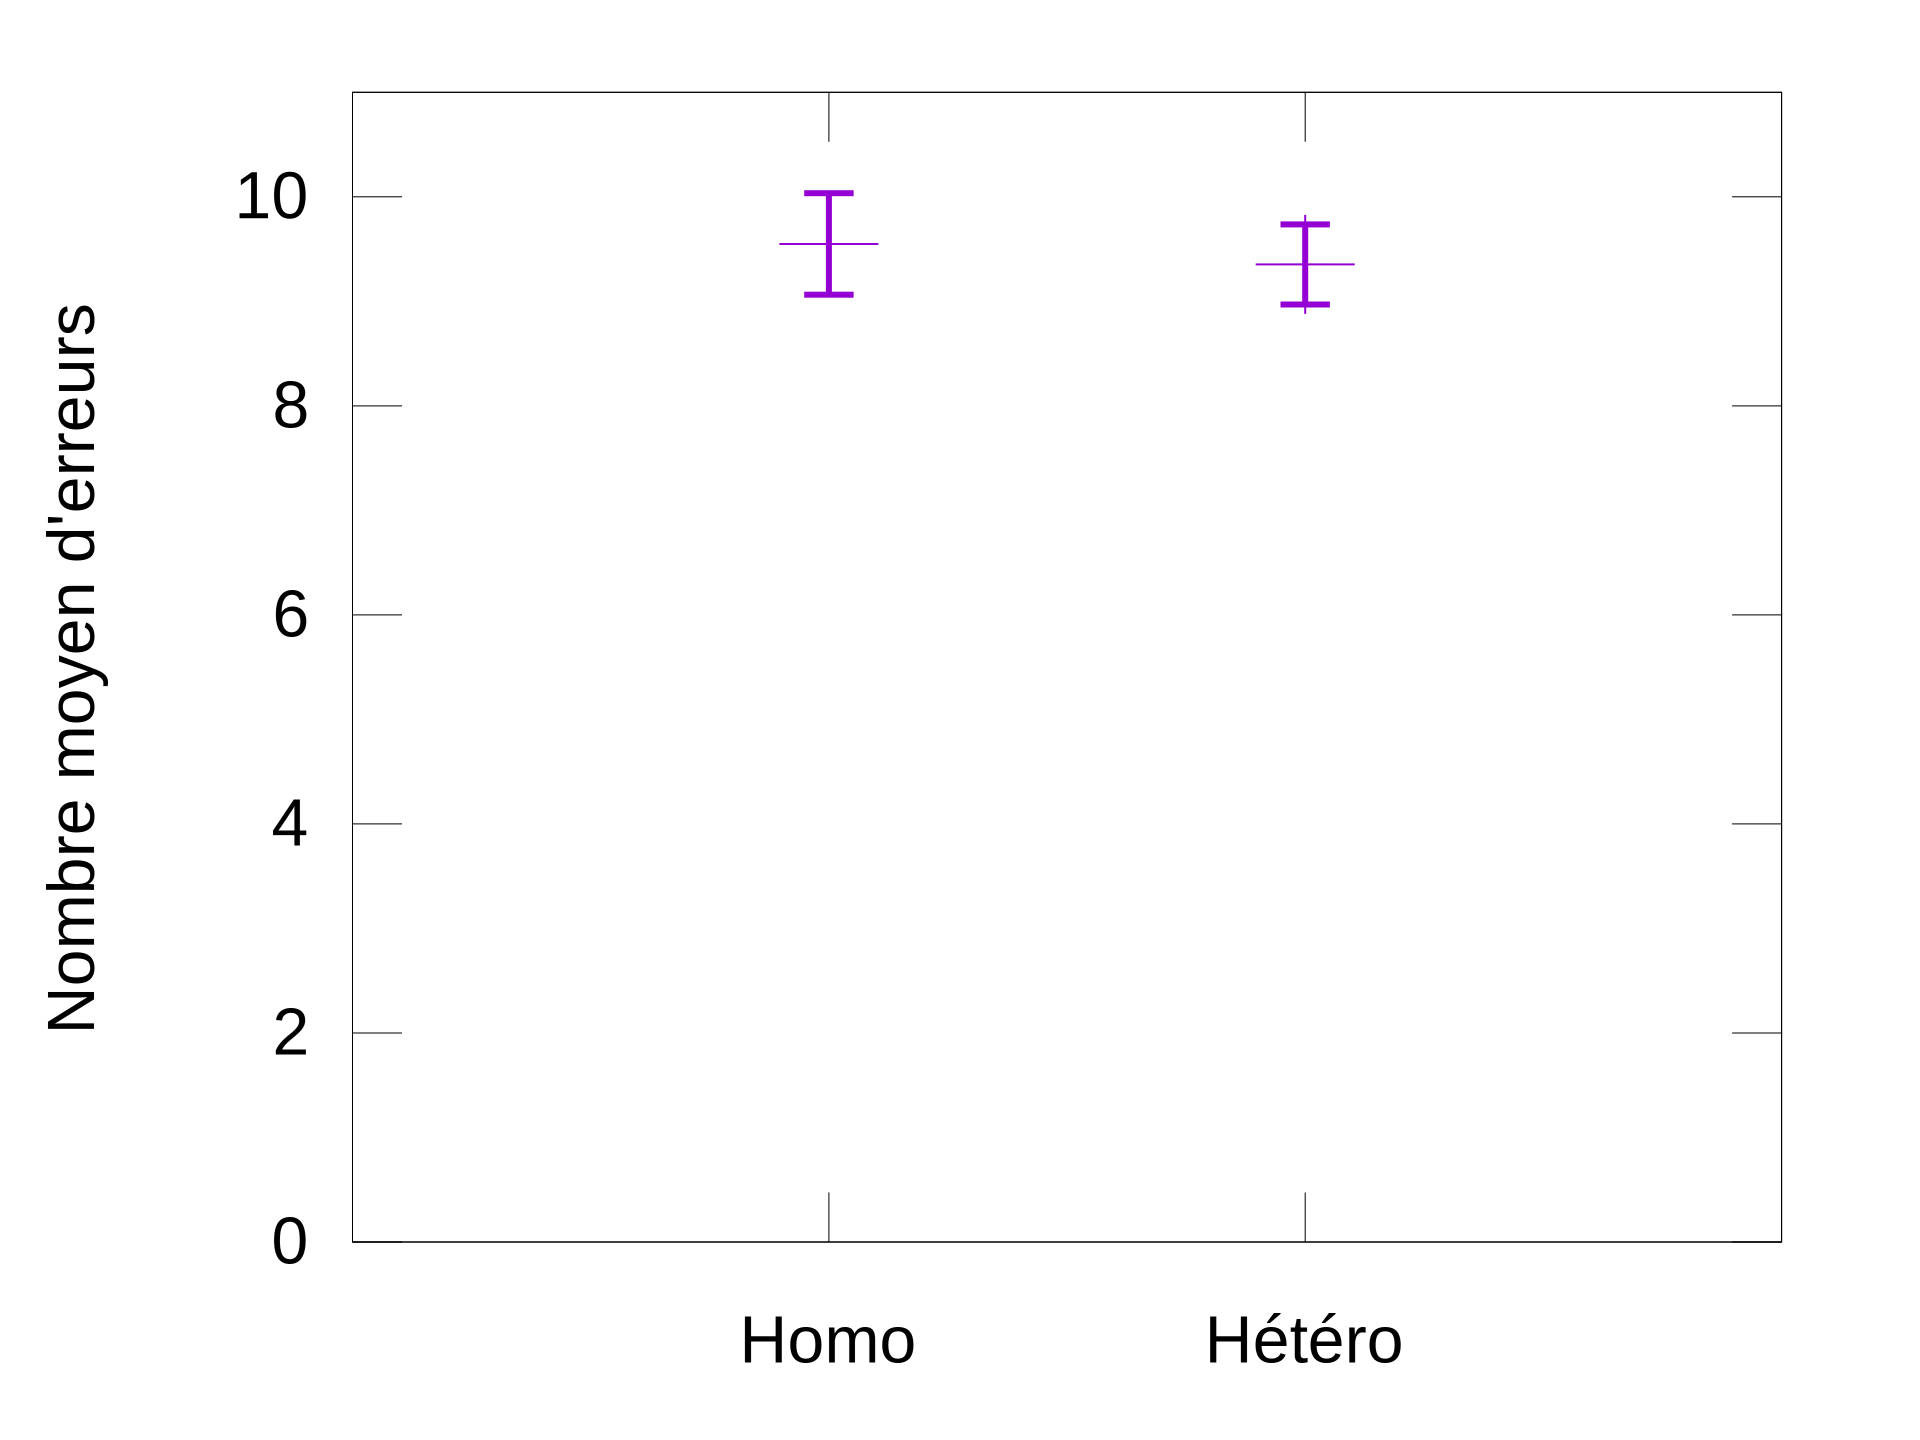
\includegraphics[width=\textwidth]{figures/ch5/errorRes}
			\caption{Nombres moyens d'erreurs, et intervalles de confiance à 95~\%{}.}
			\label{fig:errorRes}
		\end{subfigure}
		~
		\begin{subfigure}[t]{0.49\textwidth}
			\centering
			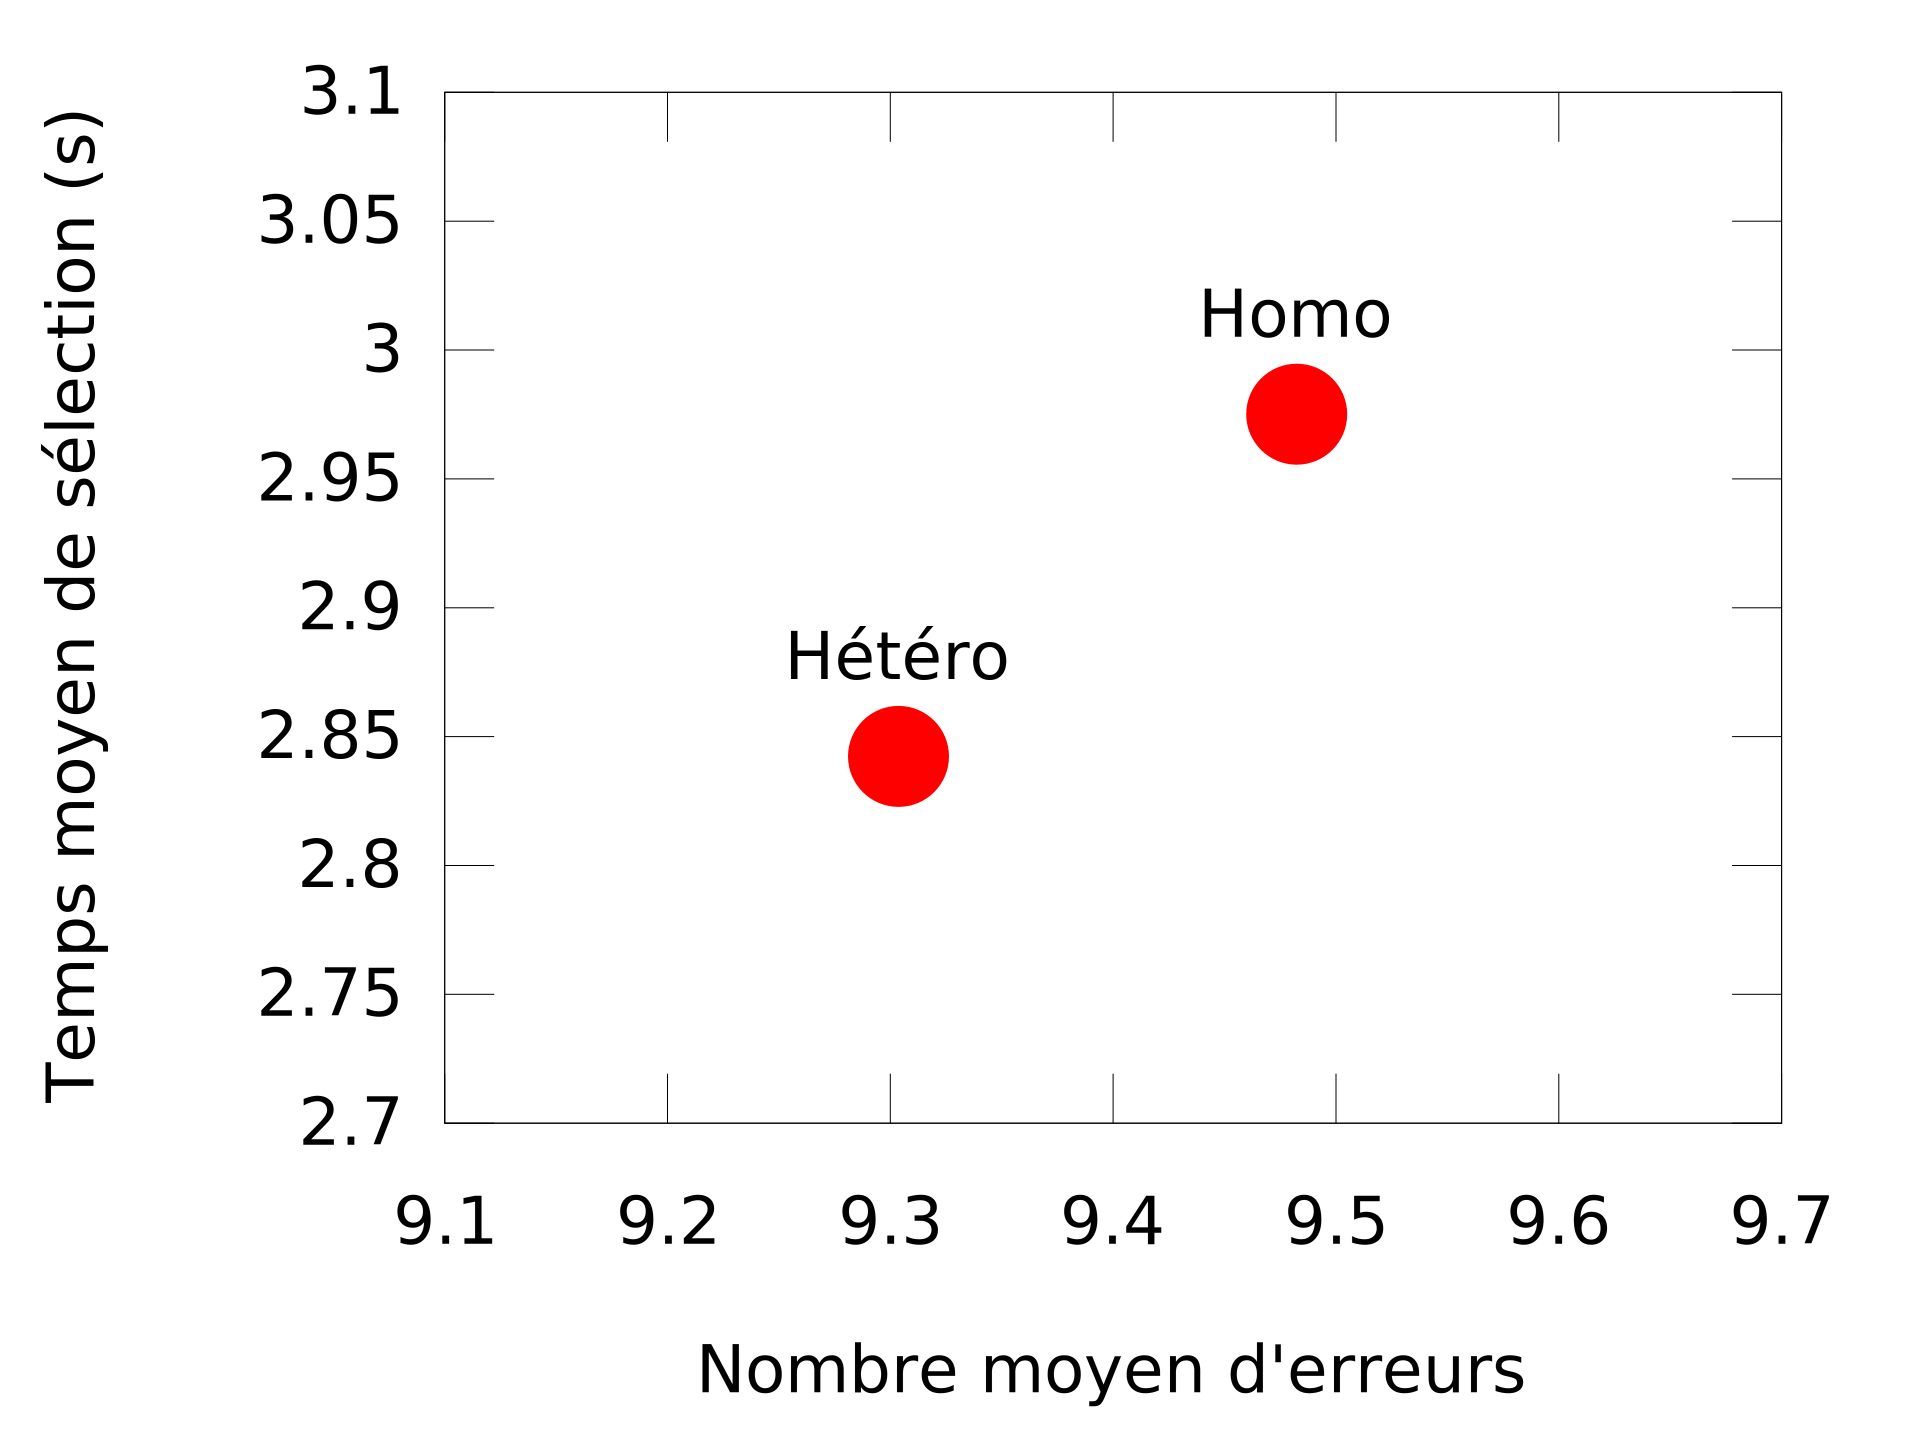
\includegraphics[width=\textwidth]{figures/ch5/errorsTimesScatter}
			\caption{Temps moyens de sélection et nombres moyens d'erreurs. Une technique \og idéale \fg{} serait située dans le coin inférieur gauche (temps courts, et peu d'erreurs), tandis qu'une technique très mauvaise serait dans le coin supérieur droit (temps longs, et beaucoup d'erreurs).}
			\label{fig:errorsTimesScatter}
		\end{subfigure}
		~
		\begin{subfigure}[t]{0.49\textwidth}
			\centering
			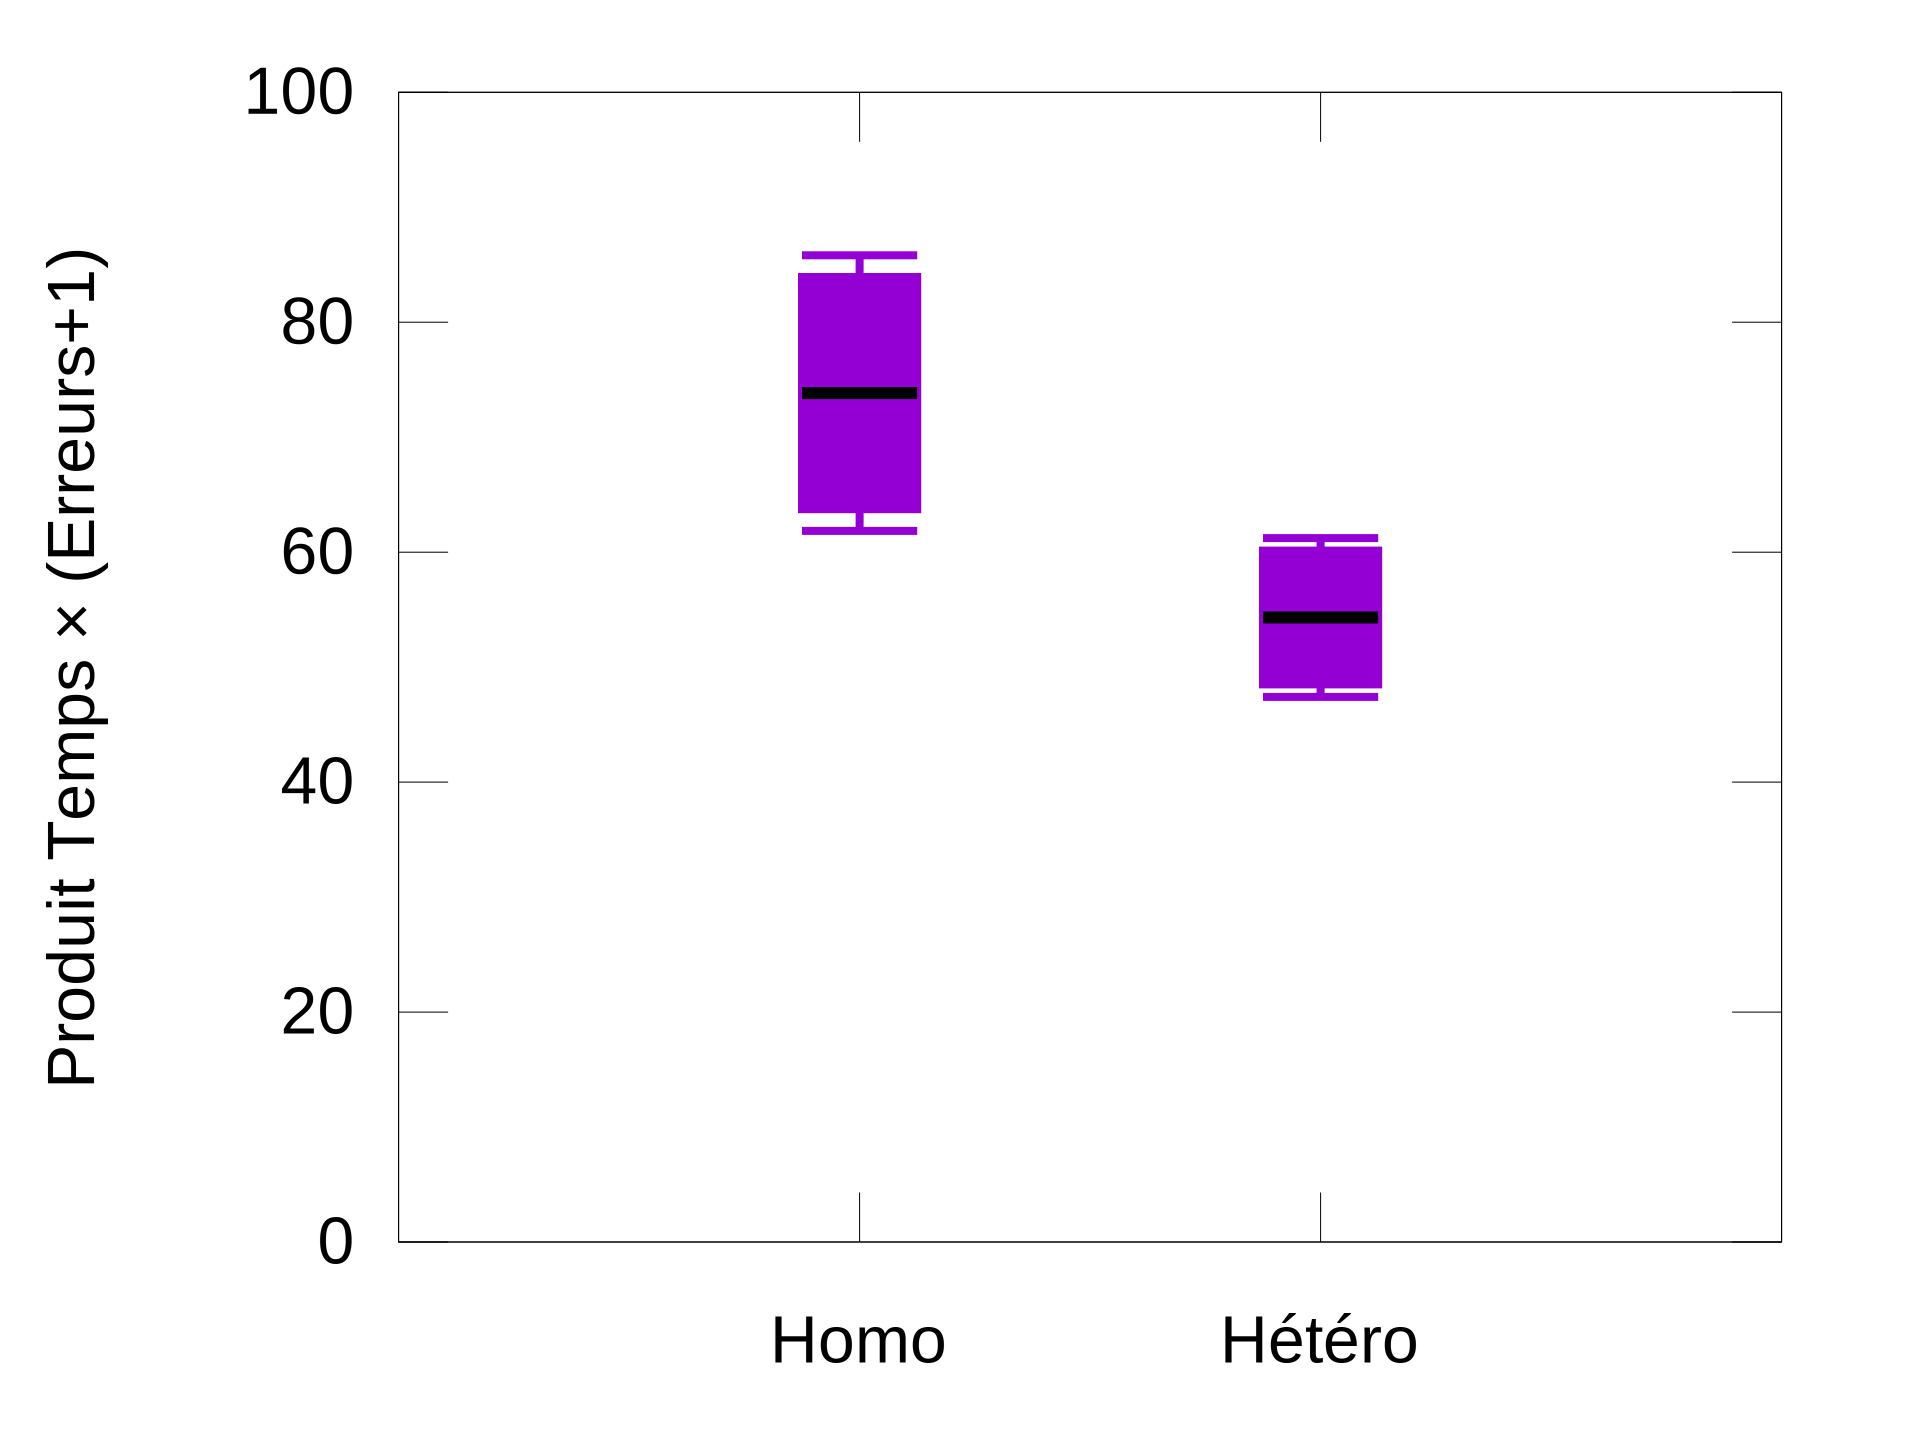
\includegraphics[width=\textwidth]{figures/ch5/productRes}
			\caption{Produit du temps de sélection par le nombre d'erreurs (plus un). Les boîtes indiquent les intervalles de confiance à 95~\%{}, les \og moustaches \fg{} à leurs extrémités indiquent les intervalles de confiance à 98~\%{}, et les barres noires horizontales, les valeurs moyennes.}
			\label{fig:productRes}
		\end{subfigure}
		\caption[Temps et erreurs de sélection, homogène vs. hétérogène]{Temps et erreurs de sélection, en condition homogène et en condition hétérogène.}
		\label{fig:timeAndErrorRes}
	\end{figure}
	
	\subsubsection{Temps de sélection}
	Dans la condition homogène, aucune corrélation significative ne fut trouvée entre le temps de sélection d'une cible et son paramètre F, ou A, comme nous pouvions nous y attendre compte tenu des interactions complexes entre les paramètres VFA.
	
	Cependant, une corrélation de 27,22~\%{} est observée entre la vitesse d'une cible et son temps de sélection, avec une \emph{p-value} de $2,19.10^{-43}$, ce qui n'est pas négligeable. Ces données confirment que la vitesse peut fournir une première approximation très grossière, mais potentiellement utile, de la difficulté de sélection d'une cible, ce qui est cohérent avec de nombreux travaux antérieurs.
	
	Mais une corrélation nettement plus forte est observée entre notre estimation de la difficulté de sélection d'une cible et son temps de sélection : 40,3~\%{}, avec une \emph{p-value} de $1,81.10^{-97}$. Notre hypothèse \textbf{H1} est donc retenue pour les temps de sélection.
	
	Il est par ailleurs intéressant d'observer que la corrélation entre la difficulté estimée et le temps de sélection est très fortement atténuée (et même inversée) dans la condition hétérogène : -7,13~\%{}, avec une \emph{p-value} inférieure à 0,0004. Ce résultat suggère que notre ajustement des tailles des cibles compense bien les écarts de difficulté\ldots{} et même un peu trop. La valeur du paramètre N choisie pour notre parabole était donc peut-être un peu trop élevée.
	
	La figure~\ref{fig:timeRes} présente les temps moyens de sélection observés dans la condition homogène d'une part, et hétérogène d'autre part. Si l'ajustement de la taille des cibles permet de diminuer le temps moyen de sélection, les intervalles de confiance à 95~\%{} ne sont pas disjoints ; aussi ne pouvons-nous retenir l'hypothèse \textbf{H2} pour les temps de sélection.
	
	\subsubsection{Erreurs}
	De même que pour les temps de sélection, dans la condition homogène, aucune corrélation significative n'est observé entre les erreurs et F ou A. En revanche, la corrélation entre la vitesse d'une cible et le nombre d'erreurs lors de sa sélection est relativement élevée : 29,95~\%{}, avec une \emph{p-value} de $1,46.10^{-52}$. Mais encore une fois, notre estimation de la difficulté fournit une meilleure corrélation : 43,02~\%{}, avec une \emph{p-value} de $2,72.10^{-112}$. Ici encore, nous observons une inversion de la corrélation dans la conditon hétérogène : -7,21~\%{}, avec une \emph{p-value} de 0,0003. Notre hypothèse \textbf{H1} est donc tout aussi valable pour les erreurs que pour les temps de sélection.
	
	La figure~\ref{fig:errorRes} présente le nombre moyen d'erreurs en fonction de la condition, homogène ou hétérogène. Là encore, si l'ajustement de la taille des cibles permet de diminuer le nombre moyen d'erreurs, les intervalles de confiance à 95~\%{} ne sont pas disjoints, de sorte que nous ne pouvons retenir l'hypothèse \textbf{H2} pour les erreurs.
	
	\subsubsection{Performances de sélection}
	Néanmoins, les performances de sélection ne sauraient être envisagées sous l'angle seul des temps de sélection, ou des erreurs. En effet, les tâches physiques en général~\cite{woodworth1899accuracy}, et le pointage en particulier~\cite{fitts1966cognitive} sont connus depuis longtemps pour être des compromis entre vitesse et précision. Ce compromis est même quantifié pour le pointage~\cite{mackenzie2008fitts, guiard2011fitt, guiard2015mathematical}, et décrit comme un compromis de type \emph{max-max} si l'on considère la vitesse et la précision, qu'il faut maximiser, ou \emph{min-min} si l'on considère, de manière équivalente, le temps de sélection et les erreurs, qu'il faut minimiser.
	
	Nous proposons donc de considérer les deux valeurs \emph{simultanément}, plutôt que séparément. C'est l'objet de la figure~\ref{fig:errorsTimesScatter}, qui présente le nombre moyen d'erreurs en abscisse, et le temps moyen de sélection en ordonnée, pour chaque condition. Le but d'une technique d'aide à la sélection peut ainsi être conçu comme le déplacement des mesures de performance vers le coin inférieur gauche, idéalement sur les deux axes. C'est ce que l'ajustement des tailles des cibles permet, quoique de manière assez faible sur chaque axe.
	
	Observons au passage que les temps de sélection et les erreurs sont naturellement très fortement corrélés, à hauteur de 90,74~\%{} dans la condition homogène, et 86,82~\%{} dans la condition hétérogène ; dans les deux cas, la \emph{p-value} est trop faible pour que nos outils puissent la distinguer de zéro. Ainsi, l'ajustement des tailles ne change pas fondamentalement la nature du compromis vitesse-précision de la tâche.
	
	\paragraph{Produit temps $\times$ erreurs.}
	Attendu que chaque composante des performances de sélection est à minimiser, nous pouvons adopter une métrique scalaire unique pour mesurer les performances : la moyenne des produits du temps de sélection par le nombre d'erreurs, pour chaque essai. Afin d'éviter d'obtenir des résultats nuls en cas d'absence d'erreur, et pour conserver le temps de sélection tel quel dans ce cas-là, nous proposons la métrique suivante : $Perf = T \times{} (E+1)$, où $Perf$ représente les performances, $T$ est le temps de sélection, et $E$ le nombre d'erreurs.
	
	Assez logiquement, il n'y a pas de corrélation significative entre $Perf$ et F, ou A, mais il y en a une entre $Perf$ et V : 19,80~\%{}, avec une \emph{p-value} de $2,39.10^{-23}$, et surtout entre $Perf$ et l'estimation de la difficulté de la cible : 29,35~\%{}, avec une \emph{p-value} de $1,77.10^{-50}$.
	
	Nous avons calculé cette valeur pour chaque essai, et en présentons les valeurs moyennes dans la figure~\ref{fig:productRes}, avec les intervalles de confiance à 95~\%{} et 98~\%{}, qui demeurent disjoints entre les conditions homogène et hétérogène, avec un net avantage pour cette dernière.
	
	Il nous apparaît donc que, sur le fondement de cette métrique de performances, inspirée des travaux sur le compromis vitesse-précision exprimé par la loi de Fitts, notre hypothèse \textbf{H2} peut être retenue, concernant les performances de sélection prises dans leur ensemble.
	
	\subsubsection{Homogénéisation des performances}
	Notre ajustement des tailles des objets mobiles ayant pour conséquence de faciliter la sélection des cibles difficile, et de rendre plus difficile la sélection des cibles faciles, il est possible de voir le procédé comme une homogénéisation des performances de sélection sur l'ensemble des cibles en présence. Dans certains types d'application, garantir (ou favoriser) une expérience d'utilisateur homogène selon les conditions rencontrées peut être vu comme une fin en soi.
	
	De fait, il est intéressant de chercher à quantifier cette homogénéisation des performances de sélection. C'est ce que fait la figure~\ref{fig:homogeneityHistogram}, qui présente lse écarts-types du temps de sélection, du nombre d'erreurs, et de $Perf$, selon la condition. Sur toutes ces métriques, l'ajustement des tailles des cibles est corrélé avec une diminution, assez marquée sur les erreurs, très marquée sur $Perf$.
	
	\begin{figure}[!htb]
		\centering
		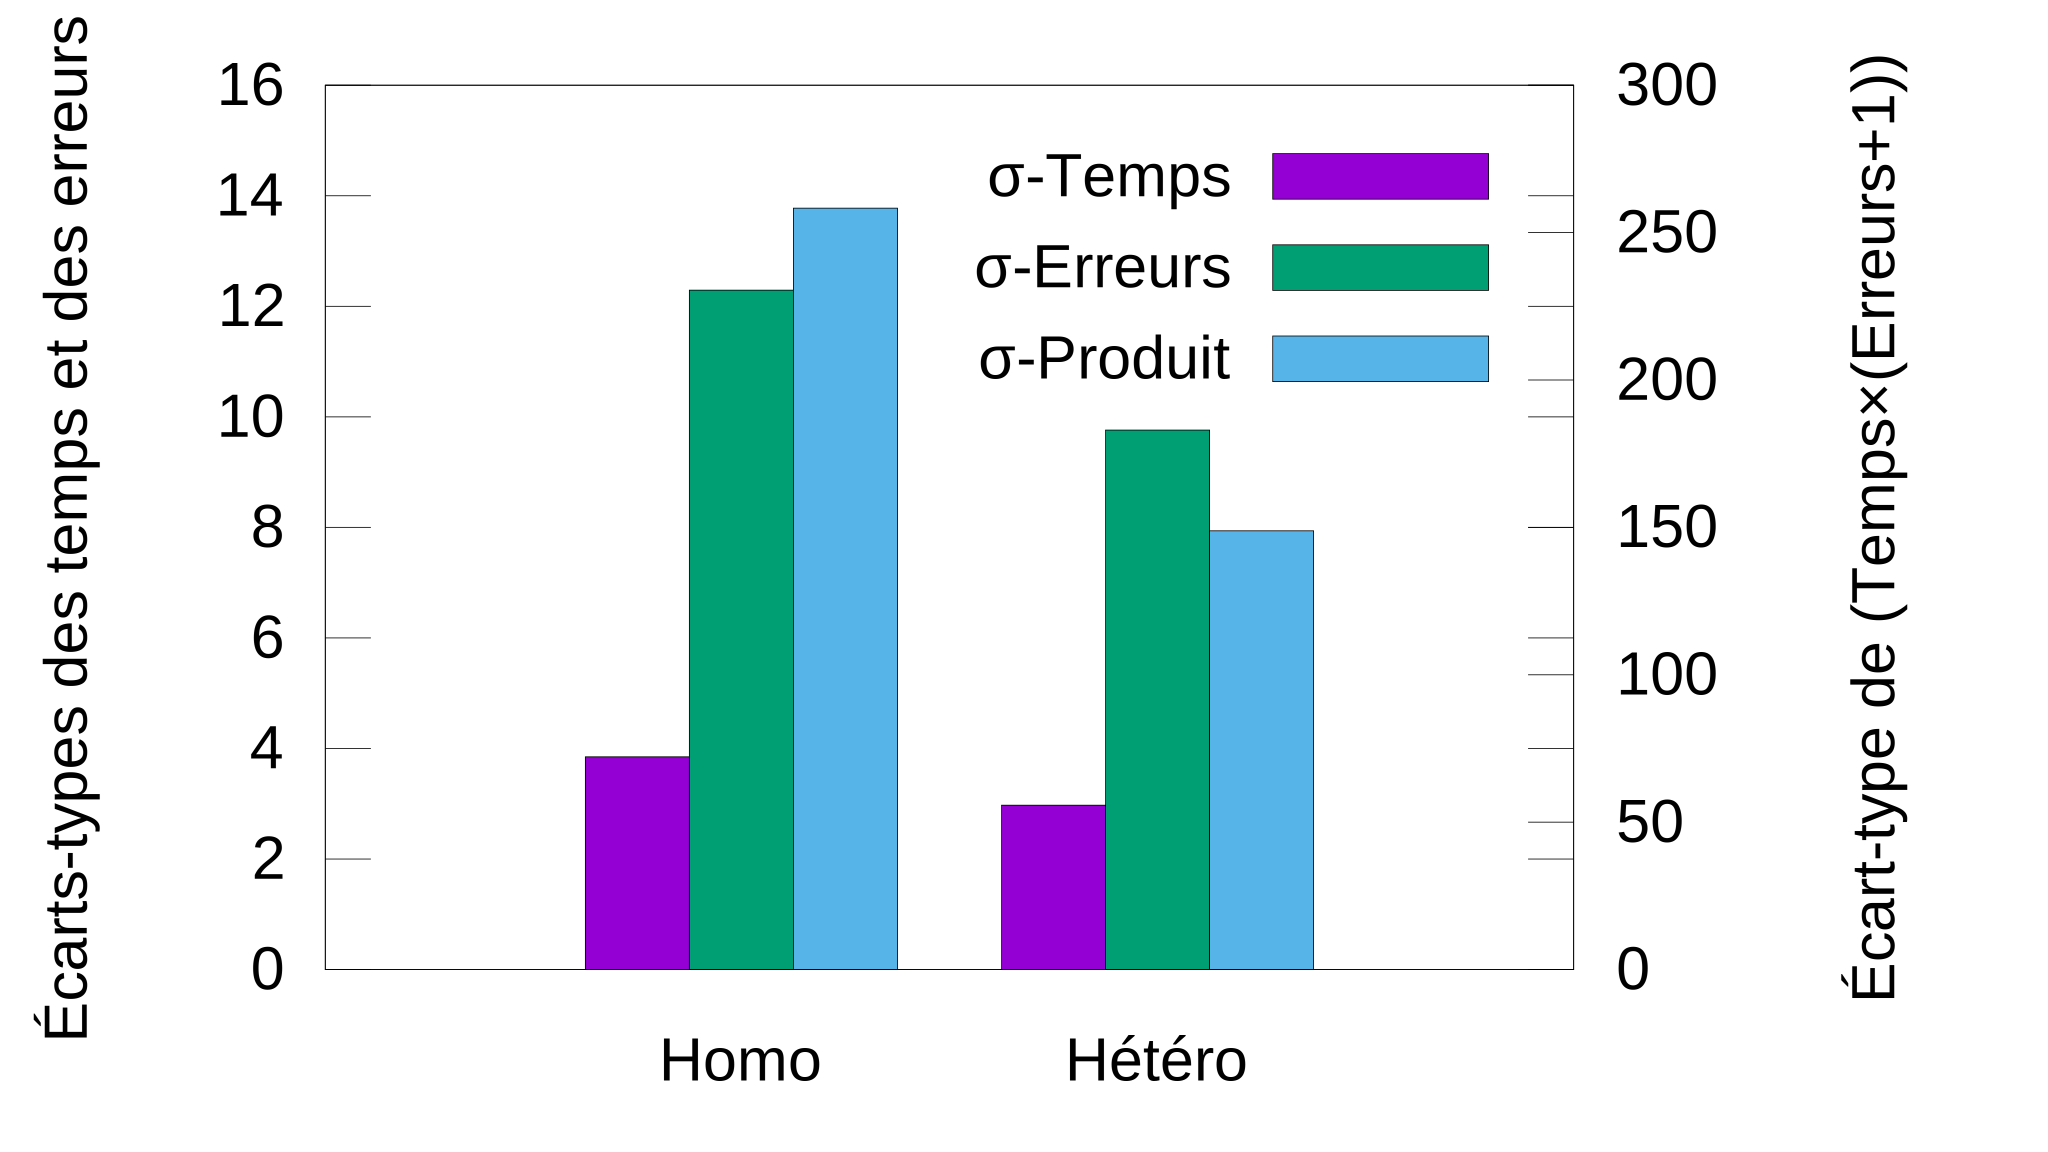
\includegraphics[width=\textwidth]{figures/ch5/homogeneityHistogram}
		\caption[Homogénéisation des performances par ajustement des tailles]{Homogénéisation des performances par ajustement des tailles des cibles. Les écarts-type du temps de sélection, du nombre d'erreurs, et du produit $Perf$ sont représentés : les deux premières valeurs sont sur l'échelle de gauche, la troisième est sur l'échelle de droite.}
		\label{fig:homogeneityHistogram}
	\end{figure}
	
	\subsubsection{Synthèse numérique des résultats}
	Nous proposons dans le tableau~\ref{tab:synthRes} une synthèse des résultats numériques de notre étude sur l'ajustement des tailles des cibles. Les valeurs de ce tableau correspondent à celles présentées graphiquement dans les sections précédentes.
	
%	\newcommand{\newrow}{\bigstrut[t] \\ \hline}
	\begin{table}
		\centering
		\begin{tabular}{l | c c}
			Condition				& Homogène						& Hétérogène			\bigstrut[b] \\ \hline
			Temps moyen				& 2,9751						& 2,8423				\bigstrut[t] \\
			Int. conf. 95~\%{}		& [2,8236 ; 3,1266]				& [2,7253 ; 2,9594]		\bigstrut[b] \\ \hline
			Erreurs					& 9,4823						& 9,3036				\bigstrut[t] \\
			Int. conf. 95~\%{}		& [8,9985 ; 9,9661]				& [8,9195 ; 9,6878]		\bigstrut[b] \\ \hline
			$Perf$ moyenne			& 74,1061						& 54,4747				\bigstrut[t] \\
			Int. conf. 95~\%{}		& [63,9409 ; 84,2713]			& [48,6160 ; 60,3335]	\\
			Int. conf. 98~\%{}		& [62,0427 ; 86,1695]			& [47,5220 ; 61,4275]	\bigstrut[b] \\ \hline
			Corr(diff, temps)		& 0,4030 ; 1,8086$.10^{-97}$	& -0,0713 ; 0,0004	\bigstrut[t] \\
			Corr(V, temps)			& 0,2722 ; 2,1890$.10^{-43}$	& -0,0518 ; 0,0099	\\
			Corr(diff, erreurs)		& 0,4302 ; 2,7188$.10^{-112}$	& -0,0721 ; 0,0003	\\
			Corr(V, erreurs)		& 0,2995 ; 1,4558$.10^{-52}$	& -0,0474 ; 0,0183	\\
			Corr(diff, $Perf$)		& 0,2935 ; 1,7719$.10^{-50}$	& -0,0378 ; 0,0599	\\
			Corr(V, $Perf$)			& 0,1980 ; 2,3853$.10^{-23}$	& -0,0302 ; 0,1326	\\
			Corr(temps, erreurs)	& 0,9074 ; --					& 0,8682 ; --			\\
			Écart-type temps		& 3,8493						& 2,9736				\\
			Écart-type erreurs		& 12,2926						& 9,7608				\\
			Écart-type $Perf$		& 258,2776						& 148,8590				\\
		\end{tabular}
		\caption[Synthèse des résultats de l'étude sur l'ajustement des tailles]{Synthèse des résultats de l'étude sur l'ajustement des tailles. Les abbréviations \og Int. conf. \fg{}, \og Corr \fg{}, et \og diff \fg{} signifient respectivement \og Intervalle de confiance à \fg{}, \og Corrélation \fg{} (accompagnée de sa \emph{p-value}), et \og estimation de la difficulté de sélection d'une cible \fg{}. Les corrélations entre la vitesse ou l'estimation de la difficulté d'une part, et le temps de sélection, les erreurs, ou $Perf$ de l'autre, qui sont marquées et significatives dans la condition homogène, disparaissent --- et même s'inversent --- dans la condition hétérogène.}
		\label{tab:synthRes}
	\end{table}
	
	\subsection{Interprétation}
	L'objet de cette étude était moins de développer une technique d'aide à la sélection de cibles mobiles que de démontrer la validité et l'utilité de notre modèle d'estimation de la difficulté d sélection d'une cible mobile. En effet, les contraintes placées étaient très fortes, et avaient pour but de tester nos hypothèses \textbf{H1} et \textbf{H2}. Nous retenons la première sans réserves, et la seconde lorsque les performances de sélection sont considérées de manière holistique, et non seulement sur le plan du temps de sélection ou du taux d'erreurs. Une tâche de sélection étant par essence un compromis vitesse-précision, il nous semble que l'hypothèse \textbf{H2} ne devrait pas être rejetée, quoique nous aimerions la voir évaluée plus précisément, avec plus de sujets, voire d'essais par sujet. Ajoutons que les inversions de corrélations notées dans le tableau~\ref{tab:synthRes} plaident pour une légère diminution du paramètre N de la parabole décrite par l'équation~\ref{eq:scalingParabola}, ce qui pourrait également améliorer les résultats.
	
	Cette étude montre qu'il est possible d'estimer de manière relativement fiable la difficulté de sélection d'une cible mobile, et de s'appuyer sur cette donnée pour informer la conception d'une technique d'assistance à la sélection. Notre proposition d'ajustement des tailles des cibles est en effet parfaitement comptabile avec un large éventail de techniques de sélection, parmi lesquelles nous pouvons citer la plupart des curseurs zonaux, comme notamment le \emph{DynaSpot}~\cite{chapuis2009dynaspot}, le lancer de rayon avec désambiguïsation~\cite{grossman2006design}, la sélection en cascade telle que la met en \oe{}uvre le \emph{Disambiguation Canvas}~\cite{debarba2013disambiguation}, par exemple, ou encore l'augmentation des objets, comme avec \emph{Comet}~\cite{hasan2011comet}, par exemple.
	
	\subsubsection{Prédiction intentionnelle biaisée}
	Au premier abord, l'ajustement des tailles des cibles pourrait paraître sans intérêt lorsque l'on utilise une heuristique de prédiction intentionnelle telle que \emph{Hook}~\cite{ortega2013hook}, qui ne se préoccuppe pas de la taille des objets. Cependant, il n'en est rien.
	
	Certes, la difficulté d'une cible due à ses mouvements n'a pas d'influence, \emph{a priori}, sur l'intention de l'utilisateur de la sélectionner ou non. Cependant, attendu qu'une heuristique de ce type s'appuie sur un système de scores pour deviner quel objet l'utilisateur cherche à sélectionner, il est possible d'utiliser la difficulté de sélection pour biaiser l'heuristique en faveur des cibles les plus difficiles, de manière tout à fait analogue à ce que nous avons fait avec la taille des cibles dans l'étude précédente. La difficulté pourrait tout simplement, à l'aide d'une parabole du type de celles de la figure~\ref{fig:parabolae}, fournir un facteur permettant de biaiser le score de la cible.
	
	Ainsi, les cibles naturellement faciles seraient certes un peu plus délicates à sélectionner, mais \emph{Hook} est suffisamment performant pour supposer que cela ne pose pas de problème, et les cibles les plus difficiles à saisir seraient plus facilement \og accrochées \fg{} par l'heuristique. Comme nous l'évoquions plus haut, \emph{Hook} est compatible avec les méthodes de filtrages décrites dans la section~\ref{sub:vfaGuide}, et l'ajustement de la taille des cibles peut s'y ajouter sans incompatibilité aucune. Notons que ce qui vaut pour \emph{Hook} et son curseur ponctuel vaut également pour \emph{IntenSelect}~\cite{de2005intenselect} et son lancer de rayon avec prédiction intentionnelle.
	
	\subsubsection{Assistance haptique ou pseudo-haptique}
	Par ailleurs, rien de tout cela n'empêche d'utiliser une assistance haptique ou pseudo-haptique, qui pourrait également dépendre du résultat final de l'heuristique de prédiction intentionnelle, c'est-à-dire à la fois de l'intention prédite, et de la difficulté des cibles potentielles. Il nous apparaît important de garder toutes ces options à l'esprit, et de les combiner au besoin, selon les difficultés et contraintes inhérentes à chaque contexte applicatif.
	
	\section{Améliorer l'estimation de la difficulté de sélection}
	Notre modèle d'estimation de la difficulté de sélection fournit des résultats cohérents et fiables, nous l'avons vu. Cependant, il n'est pas sans faiblesses, comme l'illustre par exemple la différence entre les figures~\ref{fig:perf_V_RealArea_lousy_fit} et~\ref{fig:perf_V_RealArea_better_fit}, qui met en lumière le manque de précision de notre modèle lorsque la valeur de F est particulièrement basse.
	
	Sans doute serait-il possible d'améliorer l'estimation de la difficulté de sélection d'une cible ; c'est du moins ce que suggèrent les valeurs de nos corrélations résumées par le tableau~\ref{tab:synthRes}, qui montrent une certaine marge de progression. Une modélisation mathématique plus astucieuse serait probablement utile, de même que des données plus variées et plus nombreuses à fin de l'étalonner.
	
	\subsection{Réseaux de neurones}
	Une méthode radicalement différente consisterait à employer un procédé d'apprentissage machine, tel qu'un réseau de neurones. Les entrées du réseau devraient inclure V, F, et A, voire également la largeur W et la distance D du modèle classique de Fitts, que nous avons entièrement omis dans ces travaux, en les fixant, pour limiter le focus --- déjà très large --- des études menées. Nous pourrions également y ajouter le coefficient d'autocorrélation, décrit dans la section~\ref{sub:vfaMem}. La sortie du réseau serait tout simplement une estimation de la difficulté de sélection de la cible concernée. Il est probable qu'un tel réseau, nourri de suffisamment de données d'apprentissage, fournirait une estimation nettement plus fiable, et donc potentiellement plus utile, de la difficulté inhérente à la sélection d'une cible mobile.
	
	Certes, les réseaux de neurones ont parfois l'inconvénient d'être comparables à des \og boîtes noires \fg{}, permettant difficilement de comprendre pourquoi et comment ils aboutissent à un résultat donné. En ce sens, ils pourraient être plus difficiles à appréhender pour la conception de paradigmes de sélection. Néanmoins, nous demeurons convaincus de l'intérêt de poursuivre cette piste dans de futurs travaux.
	
	\section{Conclusion}
	Dans la première partie de ce chapitre, nous avons exposé plusieurs méthodes permettant de faciliter la sélection de cibles mobiles en jouant sur leurs paramètres VFA, soit directement, soit à l'aide de \emph{proxies}, ou en lissant simplement les trajectories. Nous avons estimé quantitativement les effets de ces méthodes sur la nature des mouvements des objets concernés, et avons examiné les mérites respectifs de ces différents procédés.
	
	Nous avons proposé de mêler la prédiction intentionnelle à l'utilisation sporadique de \emph{proxies} afin de limiter l'encombrement visuel généré, et nous avons souligné l'intérêt de mêler tous ces procédés à des techniques de sélection existantes et éprouvées.
	
	Puis, dans la seconde partie du chapitre, nous avons évalué la possibilité d'utiliser l'estimation de la difficulté de sélection d'une cible pour en ajuster la taille afin d'améliorer les performances de sélection globale. Pour ce faire, nous avons mené une étude empirique avec 16 participants. Celle-ci a permis de valider l'efficacité de notre prédiction de la difficulté de sélection, et de montrer que les performances pouvaient être améliorées en ajustant les tailles des cibles, de même que l'homogénéité des performances en question.
	
	Surtout, nos résultats ouvrent de nombreuses perspectives pour le développement de paradigmes de sélection, puisqu'ils mettent en lumière la possibilité d'utiliser la difficulté de sélection d'une cible soit pour en ajuster la taille en combinaison avec une technique d'aide à la sélection efficace, soit pour biaiser une heuristique de prédiction intentionnelle\ldots{} Nous signalons par ailleurs que l'usage de tels procédés est compatible avec les procédés décrits dans la première partie du chapitre. Nous rappelons également l'intérêt potentiel de l'assistance haptique ou pseudo-haptique, qu'il est aussi possible de combiner avec les procédés sus-cités.
	
	Enfin, nous avons critiqué notre modèle de prédiction de la difficulté de sélection, et proposé une piste pour obtenir des résultats plus précis et plus fiables, afin de mieux contribuer aux performances de sélection, dans le cadre d'un paradigme combinant plusieurs procédés.

\clearpage